\documentclass[8pt]{beamer}

\usetheme[progressbar=frametitle]{metropolis}
\setbeamercolor{normal text}{bg=white}
\usepackage{appendixnumberbeamer}

\usepackage{booktabs}
\usepackage[scale=2]{ccicons}
\usepackage{multimedia}
\usepackage{pgfplots}
\usepgfplotslibrary{dateplot}
\usepackage{qrcode}
\usepackage{xspace}
\usetikzlibrary{decorations.pathreplacing}
\definecolor{stbteal}{RGB}{38,74,78}
\definecolor{stborange}{RGB}{214,111,43}
\newcommand{\themename}{\textbf{\textsc{metropolis}}\xspace}

\title{Powering SIESTA's Electronic\\
Structure Calculations with the SIESTA ToolBox}
% \date{\today}
\date{}
\subtitle{Part 2 --- Advanced STB Functions and Workflows}
\author{Dr. Carlos Maciel de Oliveira Bastos}
\institute{International Center of Physics \\ University of Brasilia}
\titlegraphic{%
	\centering
\includegraphics[height=1.2cm]{figures/banner_unb.png}%
	\begin{tikzpicture}[remember picture,overlay]
		\node[anchor=south east,xshift=-0.35cm,yshift=0.35cm]
			at (current page.south east)
			{
\includegraphics[width=2.2cm]{figures/seedmol.png}};
	\end{tikzpicture}%
}

% h-BN chain used in the adsorption slides: \hbnlayer{x}{y}
\newcommand{\hbnlayer}[2]{%
	\foreach \i in {0,...,6}{
		\pgfmathsetmacro{\xx}{#1-1.2+0.4*\i}
		\ifodd\i \node[n] at (\xx,#2) {}; \else \node[b] at (\xx,#2) {}; \fi
	}
	\draw[gray!60] (#1-1.2,#2) -- (#1+1.2,#2);
}

% recap figure tile for the closing section
\newcommand{\recapfig}[2]{%
	\begin{minipage}[t]{0.32\textwidth}\centering
		\includegraphics[width=\linewidth,height=2.55cm,keepaspectratio]{figures/#1}\\[-1pt]
		{\scriptsize\color{stbteal}#2}
	\end{minipage}}
\begin{document}

\maketitle


%-------------------------------------------------
% SLIDE 2.1.1 - Where we stopped
%-------------------------------------------------
\begin{frame}{Where We Stopped}
	\centering
	{\large\bfseries\color{stbteal}Single tool}\par\vspace{0.15cm}
	\resizebox{0.9\textwidth}{!}{%
	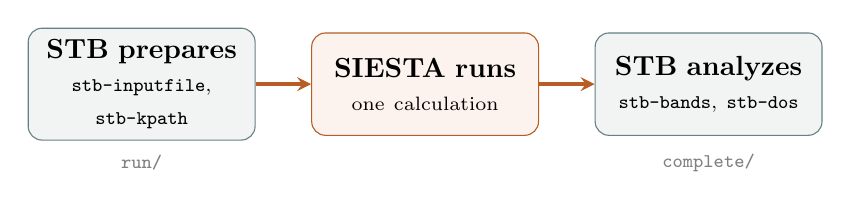
\begin{tikzpicture}[
		stb/.style={draw=stbteal!70,fill=stbteal!6,rounded corners=5pt,
			text width=2.6cm,minimum height=1.3cm,align=center,inner sep=4pt},
		run/.style={stb,draw=stborange!85!black,fill=stborange!8},
		flow/.style={->,>=stealth,line width=1.2pt,draw=stborange!85!black}
	]
		\node[stb] (a) at (0,0) {{\bfseries STB prepares}\\{\scriptsize \texttt{stb-inputfile}, \texttt{stb-kpath}}};
		\node[run] (b) at (3.6,0) {{\bfseries SIESTA runs}\\{\scriptsize one calculation}};
		\node[stb] (c) at (7.2,0) {{\bfseries STB analyzes}\\{\scriptsize \texttt{stb-bands}, \texttt{stb-dos}}};
		\draw[flow] (a) -- (b); \draw[flow] (b) -- (c);
		\node[font=\scriptsize,text=gray] at (0,-1.0) {\texttt{run/}};
		\node[font=\scriptsize,text=gray] at (7.2,-1.0) {\texttt{complete/}};
	\end{tikzpicture}%
	}
	\par\vspace{0.45cm}
	{\large\bfseries\color{stborange!85!black}Workflow}\par\vspace{0.15cm}
	\resizebox{\textwidth}{!}{%
	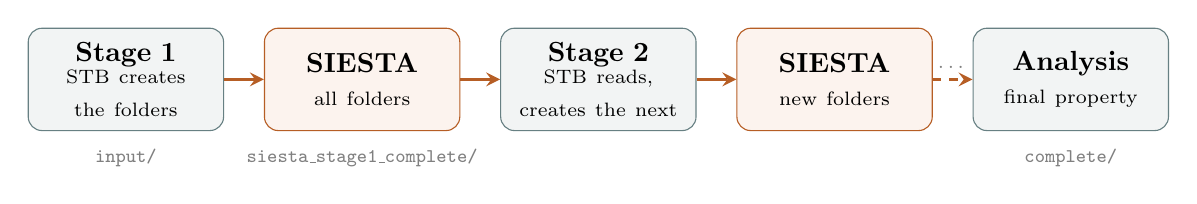
\begin{tikzpicture}[
		stb/.style={draw=stbteal!70,fill=stbteal!6,rounded corners=5pt,
			text width=2.2cm,minimum height=1.3cm,align=center,inner sep=4pt},
		run/.style={stb,draw=stborange!85!black,fill=stborange!8},
		flow/.style={->,>=stealth,line width=1.2pt,draw=stborange!85!black}
	]
		\node[stb] (a) at (0,0) {{\bfseries Stage 1}\\{\scriptsize STB creates\\the folders}};
		\node[run] (b) at (3.0,0) {{\bfseries SIESTA}\\{\scriptsize all folders}};
		\node[stb] (c) at (6.0,0) {{\bfseries Stage 2}\\{\scriptsize STB reads,\\creates the next}};
		\node[run] (d) at (9.0,0) {{\bfseries SIESTA}\\{\scriptsize new folders}};
		\node[stb] (e) at (12.0,0) {{\bfseries Analysis}\\{\scriptsize final property}};
		\draw[flow] (a) -- (b); \draw[flow] (b) -- (c); \draw[flow] (c) -- (d);
		\draw[flow,dashed] (d) -- node[above,font=\scriptsize,text=gray]{\dots} (e);
		\node[font=\scriptsize,text=gray] at (0,-1.0) {\texttt{input/}};
		\node[font=\scriptsize,text=gray] at (3.0,-1.0) {\texttt{siesta\_stage1\_complete/}};
		\node[font=\scriptsize,text=gray] at (12.0,-1.0) {\texttt{complete/}};
	\end{tikzpicture}%
	}
\end{frame}





%%%%%%%%%%%%%%%%%%%%%%%%%%%%%%%%%%%%%%%%%%%%%%%%%%%%%%%%
\section{Bands and Density of States}
%%%%%%%%%%%%%%%%%%%%%%%%%%%%%%%%%%%%%%%%%%%%%%%%%%%%%%%%

%-------------------------------------------------
% SLIDE 2.2.1 - Theory: Bloch states and the BZ
%-------------------------------------------------
\begin{frame}{Bloch Electrons and the Brillouin Zone}
	\begin{columns}[T]
		\begin{column}{0.50\textwidth}
			\metroset{block=fill}
			\begin{block}{Periodicity labels every state by $\mathbf{k}$}
				\vspace{-0.2cm}
				\begin{align*}
					\psi_{n\mathbf{k}}(\mathbf{r}) &= e^{i\mathbf{k}\cdot\mathbf{r}}\,u_{n\mathbf{k}}(\mathbf{r})\\
					u_{n\mathbf{k}}(\mathbf{r}+\mathbf{R}) &= u_{n\mathbf{k}}(\mathbf{r})
				\end{align*}
				\vspace{-0.4cm}
				\begin{itemize}
					\item $\mathbf{k}$ lives in the first Brillouin zone (BZ)
					\item For each $\mathbf{k}$, Kohn--Sham gives a ladder of levels $\varepsilon_n(\mathbf{k})$
					\item A \textbf{band} is $\varepsilon_n(\mathbf{k})$ followed continuously in $\mathbf{k}$
				\end{itemize}
			\end{block}
			\vspace{0.1cm}
			\begin{alertblock}{Two different uses of $\mathbf{k}$}
				\textbf{SCF mesh}: a uniform grid that integrates the density.\\
				\textbf{Band path}: lines through high-symmetry points, for plotting.
			\end{alertblock}
		\end{column}
		\begin{column}{0.48\textwidth}
			\centering
			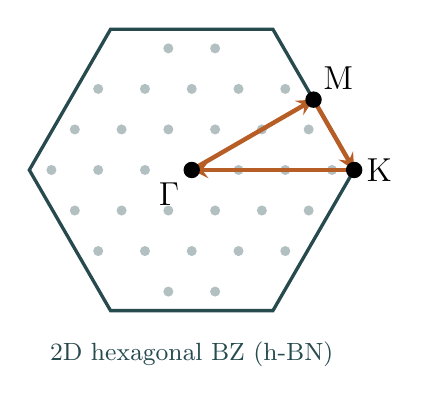
\begin{tikzpicture}[scale=1.65]
				% uniform SCF mesh (schematic)
				\foreach \i in {-4,...,4}
					\foreach \j in {-4,...,4}
					{
						\pgfmathsetmacro{\x}{0.36*\i + 0.18*\j}
						\pgfmathsetmacro{\y}{0.312*\j}
						\pgfmathparse{abs(\x)<1.25 && abs(\y)<1.08 && abs(0.5*\x+0.866*\y)<1.08 && abs(-0.5*\x+0.866*\y)<1.08 ? 1 : 0}
						\ifnum\pgfmathresult=1
							\fill[stbteal!35] (\x,\y) circle (1.1pt);
						\fi
					}
				% hexagonal BZ
				\draw[stbteal,line width=1.2pt]
					(0:1.25) -- (60:1.25) -- (120:1.25) -- (180:1.25)
					-- (240:1.25) -- (300:1.25) -- cycle;
				% path Gamma-M-K-Gamma
				\coordinate (G) at (0,0);
				\coordinate (M) at (30:1.0825);
				\coordinate (K) at (0:1.25);
				\draw[stborange!85!black,line width=1.6pt,->,>=stealth] (G) -- (M);
				\draw[stborange!85!black,line width=1.6pt,->,>=stealth] (M) -- (K);
				\draw[stborange!85!black,line width=1.6pt,->,>=stealth] (K) -- (G);
				\fill[black] (G) circle (1.8pt) node[below left=1pt] {\large$\Gamma$};
				\fill[black] (M) circle (1.8pt) node[above right=0pt] {\large M};
				\fill[black] (K) circle (1.8pt) node[right=1pt] {\large K};
				\node[font=\small,text=stbteal] at (0,-1.42) {2D hexagonal BZ (h-BN)};
			\end{tikzpicture}
			\par\vspace{0.15cm}
			{\small
			\textcolor{stbteal}{$\bullet$} SCF mesh ($15{\times}15{\times}1$, schematic)\par
			\textcolor{stborange!85!black}{\textbf{---}} band path $\Gamma$--M--K--$\Gamma$\par
			\vspace{0.15cm}
			In 2D: one k point along $z$,\\ a path in the plane.\par}
		\end{column}
	\end{columns}
\end{frame}

%-------------------------------------------------
% SLIDE 2.2.2 - Theory: reading a band structure
%-------------------------------------------------
\begin{frame}{Reading a Band Structure}
	\centering
	\resizebox{0.92\textwidth}{!}{%
	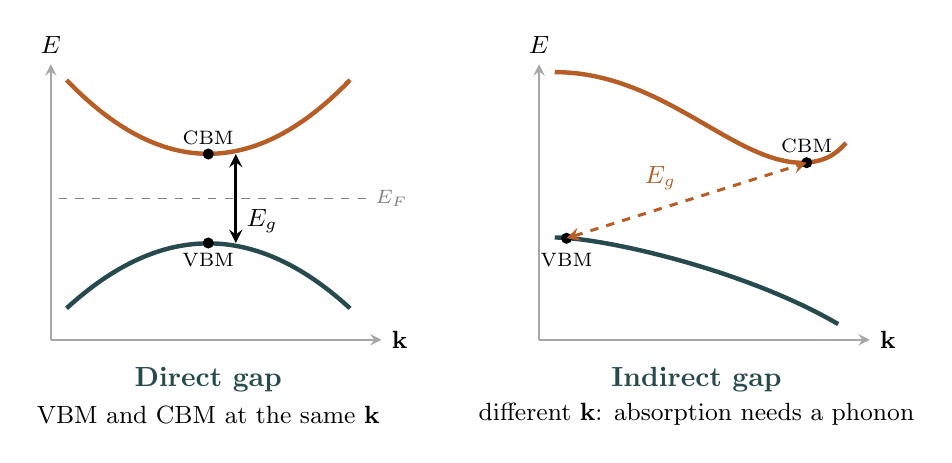
\begin{tikzpicture}[
		vb/.style={stbteal,line width=1.6pt},
		cb/.style={stborange!85!black,line width=1.6pt},
		axis/.style={->,>=stealth,draw=gray!70,line width=0.8pt},
		gap/.style={<->,>=stealth,line width=1.1pt}
	]
		% --- direct gap
		\begin{scope}
			\draw[axis] (0,-1.5) -- (0,2.0) node[above,font=\small] {$E$};
			\draw[axis] (0,-1.5) -- (4.2,-1.5) node[right,font=\small] {$\mathbf{k}$};
			\draw[vb] (0.2,-1.1) .. controls (1.4,0.0) and (2.6,0.0) .. (3.8,-1.1);
			\draw[cb] (0.2,1.8) .. controls (1.4,0.55) and (2.6,0.55) .. (3.8,1.8);
			\fill (2,-0.27) circle (2pt) node[below,font=\scriptsize] {VBM};
			\fill (2,0.86) circle (2pt) node[above,font=\scriptsize] {CBM};
			\draw[gap] (2.35,-0.27) -- (2.35,0.86) node[pos=0.25,right,font=\small] {$E_g$};
			\draw[gray,dashed] (0.1,0.3) -- (4.0,0.3) node[right,font=\scriptsize,text=gray] {$E_F$};
			\node[font=\bfseries\color{stbteal}] at (2,-2.0) {Direct gap};
			\node[font=\small] at (2,-2.45) {VBM and CBM at the same $\mathbf{k}$};
		\end{scope}
		% --- indirect gap
		\begin{scope}[xshift=6.2cm]
			\draw[axis] (0,-1.5) -- (0,2.0) node[above,font=\small] {$E$};
			\draw[axis] (0,-1.5) -- (4.2,-1.5) node[right,font=\small] {$\mathbf{k}$};
			\draw[vb] (0.2,-0.2) .. controls (0.8,-0.2) and (2.6,-0.6) .. (3.8,-1.3);
			\draw[cb] (0.2,1.9) .. controls (1.6,1.9) and (2.5,0.7) .. (3.4,0.75) .. controls (3.7,0.78) and (3.8,0.9) .. (3.9,1.0);
			\fill (0.35,-0.21) circle (2pt) node[below=2pt,font=\scriptsize] {VBM};
			\fill (3.4,0.75) circle (2pt) node[above,font=\scriptsize] {CBM};
			\draw[gap,stborange!85!black,dashed] (0.35,-0.21) -- (3.4,0.75) node[midway,above left,font=\small] {$E_g$};
			\node[font=\bfseries\color{stbteal}] at (2,-2.0) {Indirect gap};
			\node[font=\small] at (2,-2.45) {different $\mathbf{k}$: absorption needs a phonon};
		\end{scope}
	\end{tikzpicture}%
	}
	\vspace{0.2cm}
	\begin{columns}[T]
		\begin{column}{0.48\textwidth}
			\metroset{block=fill}
			\begin{block}{What the diagram tells you}
				\small
				\begin{itemize}
					\item Metal or insulator; size and type of $E_g$
					\item Band width: localized vs delocalized states
					\item Curvature: $1/m^* = \hbar^{-2}\,\partial^2 E/\partial k^2$
				\end{itemize}
			\end{block}
		\end{column}
		\begin{column}{0.48\textwidth}
			\metroset{block=fill}
			\begin{alertblock}{Kohn--Sham gap $\neq$ optical gap}
				\small
				\begin{itemize}
					\item PBE underestimates $E_g$
					\item GaAs: 0.36~eV (PBE) vs 1.42~eV (exp.)
					\item Trust trends and band character more than the number
				\end{itemize}
			\end{alertblock}
		\end{column}
	\end{columns}
\end{frame}

%-------------------------------------------------
% SLIDE 2.2.3 - Theory: DOS and PDOS
%-------------------------------------------------
\begin{frame}{Density of States and Orbital Projections}
	\begin{columns}[T]
		\begin{column}{0.42\textwidth}
			\metroset{block=fill}
			\begin{block}{Count states per energy}
				\[
					g(E) = \sum_{n}\sum_{\mathbf{k}} w_{\mathbf{k}}\,
					\delta\!\left(E-\varepsilon_{n\mathbf{k}}\right)
				\]
				{\scriptsize The $\delta$ is replaced by a peak of finite width.}
			\end{block}
			\vspace{0.05cm}
			\begin{block}{Project onto atomic orbitals $\mu$}
				\[
					\begin{aligned}
					g_\mu(E) = \sum_{n\mathbf{k}} w_{\mathbf{k}}\,
					&\mathrm{Re}\!\left[c^{*}_{\mu,n\mathbf{k}}\,(\mathbf{S}\,\mathbf{c}_{n\mathbf{k}})_\mu\right]\\
					&\times\delta\!\left(E-\varepsilon_{n\mathbf{k}}\right)
					\end{aligned}
				\]
				{\scriptsize Natural in LCAO: SIESTA already works in the orbital basis.
				$\sum_\mu g_\mu = g$.}
			\end{block}
		\end{column}
		\begin{column}{0.56\textwidth}
			\centering
			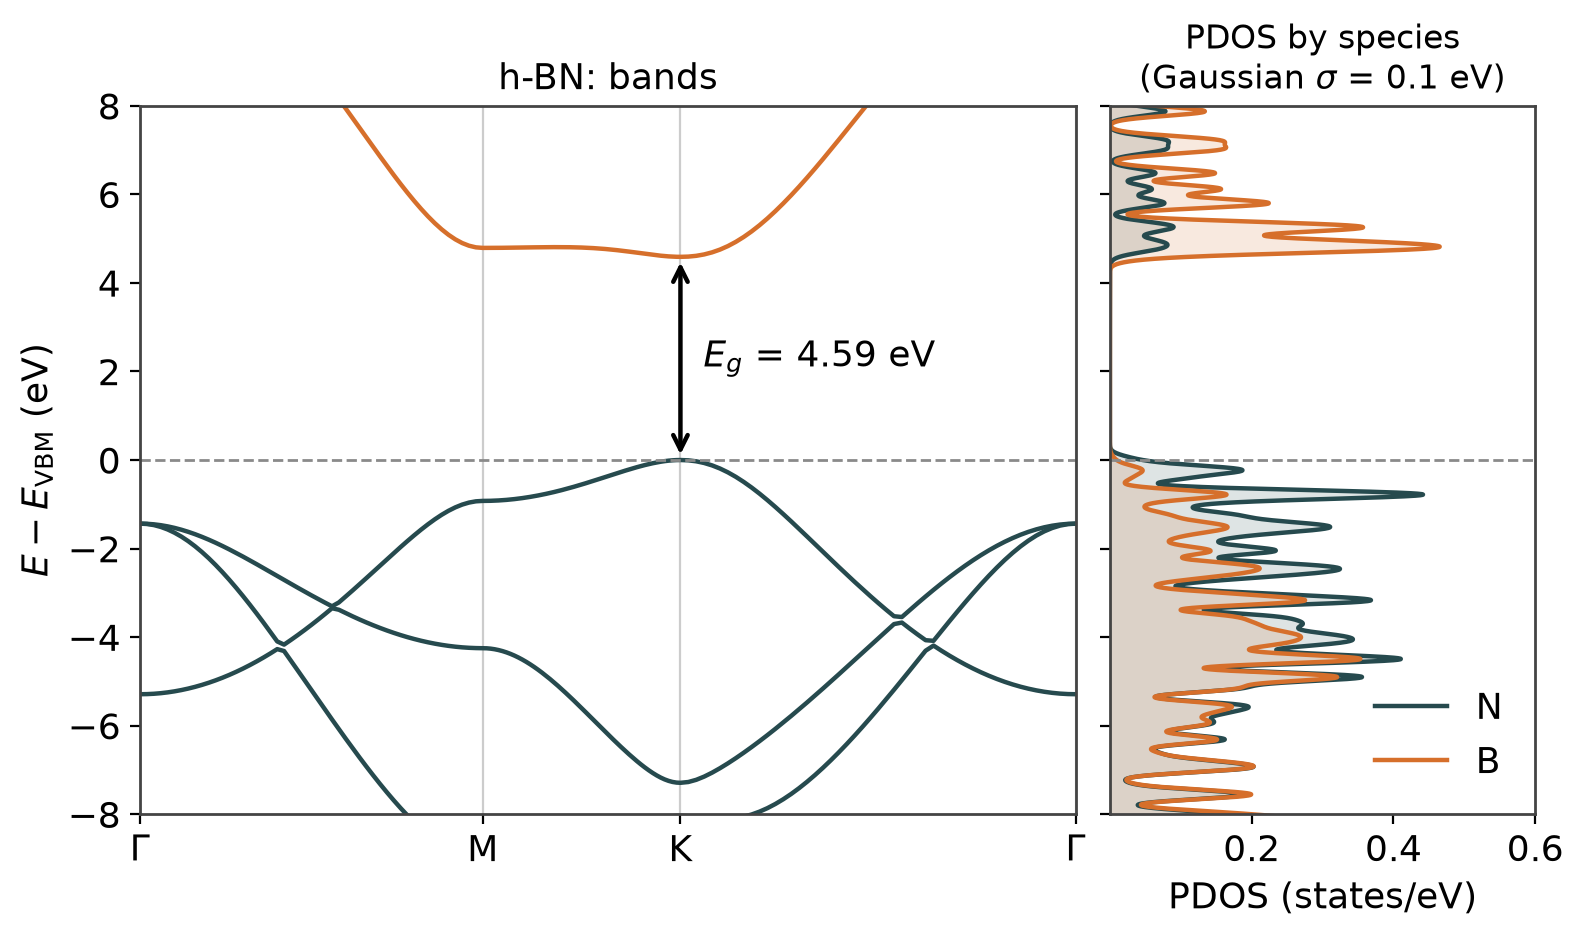
\includegraphics[width=\textwidth]{figures/hbn_bands_pdos.png}
			\par\vspace{0.1cm}
			{\small h-BN (PBE/DZP): valence band mostly N,\\ conduction band mostly B.}
		\end{column}
	\end{columns}
	\vspace{0.15cm}
	\metroset{block=fill}
	\begin{alertblock}{DOS needs the whole BZ, not the path}
		\small
		\begin{itemize}
			\item Integrated on its own uniform grid, \texttt{PDOS.kgrid\_Monkhorst\_Pack},
				usually denser than the SCF mesh
			\item DOS peaks come from flat regions of $\varepsilon_n(\mathbf{k})$
		\end{itemize}
	\end{alertblock}
\end{frame}

%-------------------------------------------------
% SLIDE 2.2.4 - How to do it in STB
%-------------------------------------------------
\begin{frame}{Bands and DOS with STB}
	\centering
	\resizebox{1.0\textwidth}{!}{%
	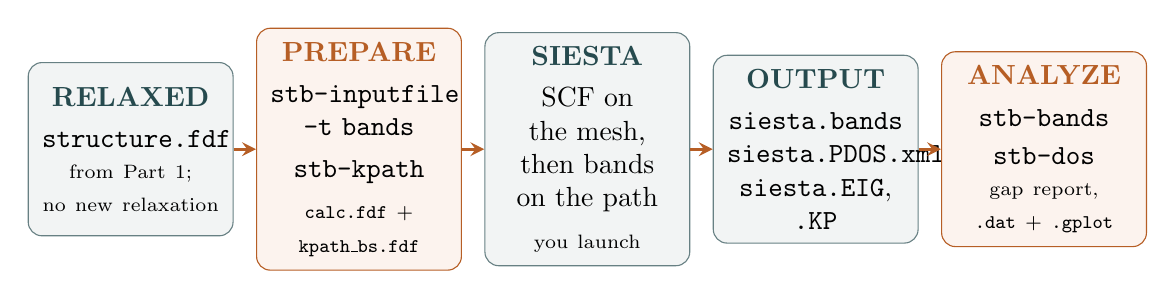
\begin{tikzpicture}[
		stage/.style={
			draw=stbteal!70,fill=stbteal!6,rounded corners=5pt,
			text width=2.25cm,minimum height=2.2cm,align=center,inner sep=5pt
		},
		tool/.style={stage,draw=stborange!85!black,fill=stborange!8},
		flow/.style={->,>=stealth,line width=1.2pt,draw=stborange!85!black}
	]
		\node[stage] (s) at (0,0) {
			{\color{stbteal}\bfseries RELAXED}\\[3pt]
			\texttt{structure.fdf}\\[3pt]
			{\scriptsize from Part 1;\\no new relaxation}
		};
		\node[tool] (inp) at (2.9,0) {
			{\color{stborange!85!black}\bfseries PREPARE}\\[3pt]
			\texttt{stb-inputfile}\\\texttt{-t bands}\\[3pt]
			\texttt{stb-kpath}\\[3pt]
			{\scriptsize \texttt{calc.fdf} + \texttt{kpath\_bs.fdf}}
		};
		\node[stage] (run) at (5.8,0) {
			{\color{stbteal}\bfseries SIESTA}\\[3pt]
			SCF on the mesh,\\then bands on the path\\[3pt]
			{\scriptsize you launch}
		};
		\node[stage] (out) at (8.7,0) {
			{\color{stbteal}\bfseries OUTPUT}\\[3pt]
			\texttt{siesta.bands}\\
			\texttt{siesta.PDOS.xml}\\
			\texttt{siesta.EIG}, \texttt{.KP}
		};
		\node[tool] (ana) at (11.6,0) {
			{\color{stborange!85!black}\bfseries ANALYZE}\\[3pt]
			\texttt{stb-bands}\\[2pt]
			\texttt{stb-dos}\\[3pt]
			{\scriptsize gap report,\\\texttt{.dat} + \texttt{.gplot}}
		};
		\draw[flow] (s) -- (inp);
		\draw[flow] (inp) -- (run);
		\draw[flow] (run) -- (out);
		\draw[flow] (out) -- (ana);
	\end{tikzpicture}%
	}
	\vspace{0.3cm}
	\begin{columns}[T]
		\begin{column}{0.5\textwidth}
			\metroset{block=fill}
			\begin{block}{What \texttt{-t bands} adds to \texttt{calc.fdf}}
				\ttfamily\scriptsize
				\%include kpath\_bs.fdf\\
				\%block ProjectedDensityOfStates\\
				\ \ -20.0 20.0 0.01 8000 eV\\
				\%endblock ProjectedDensityOfStates\\
				\%PDOS.kgrid\_Monkhorst\_Pack \ldots
			\end{block}
		\end{column}
		\begin{column}{0.46\textwidth}
			\metroset{block=fill}
			\begin{alertblock}{One run, two products}
				\small
				\begin{itemize}
					\item Path eigenvalues: \texttt{siesta.bands}
					\item Projected DOS: \texttt{siesta.PDOS.xml}
					\item Both shifted to the same VBM
				\end{itemize}
			\end{alertblock}
		\end{column}
	\end{columns}
\end{frame}

%-------------------------------------------------
% SLIDE 2.2.5 - stb-kpath
%-------------------------------------------------
\begin{frame}[fragile]{\texttt{stb-kpath}: The High-Symmetry Path}
	\begin{columns}[T]
		\begin{column}{0.48\textwidth}
			\metroset{block=fill}
			\begin{block}{What it does}
				\small
				\begin{itemize}
					\item Detects 2D/3D: an empty span $>10$~\AA\ is a vacuum axis
					\item Finds the Bravais lattice (ASE)
					\item Writes the Setyawan--Curtarolo path as a \texttt{BandLines} block
				\end{itemize}
			\end{block}
			\vspace{0.1cm}
			\begin{block}{Command and h-BN report}
				\small
\begin{verbatim}
stb-kpath -f structure.fdf --save-report
# -> kpath_bs.fdf (BandLines)
\end{verbatim}
				\vspace{-0.1cm}
				{\ttfamily
				\begin{tabular}{@{}l@{\,:\,}l}
					Dimensionality & 2D\\
					Bravais lattice & HEX2D\\
					Path & $\Gamma$-M-K-$\Gamma$
				\end{tabular}}
			\end{block}
		\end{column}
		\begin{column}{0.48\textwidth}
			\metroset{block=fill}
			\begin{alertblock}{Pitfall: noise breaks symmetry}
				\small
				Relaxed GaAs is cubic only to $\sim10^{-3}$~\AA.
				\par\vspace{0.2cm}
				\textbf{Default} \texttt{-p 0.0002} $\rightarrow$ \textbf{rhombohedral}\\
				{\small\ttfamily $\Gamma$-L-B1-B-Z-$\Gamma$-X-Q-F-P1-Z-L-P}
				\par\vspace{0.2cm}
				\textbf{Our example} \texttt{-p 0.01} $\rightarrow$ \textbf{FCC}\\
				{\small\ttfamily $\Gamma$-X-W-K-$\Gamma$-L-U-W-L-K | U-X}
			\end{alertblock}
			\vspace{0.1cm}
			\begin{block}{Before running SIESTA}
				\small
				Check the reported lattice and space group\\
				(GaAs: F$\bar{4}$3m, No.\ 216).
			\end{block}
		\end{column}
	\end{columns}
\end{frame}

%-------------------------------------------------
% SLIDE 2.2.6 - stb-bands
%-------------------------------------------------
\begin{frame}[fragile]{\texttt{stb-bands}: Gap, Character, and Plot}
	\begin{columns}[T]
		\begin{column}{0.44\textwidth}
			\metroset{block=fill}
			\begin{block}{Command}
				\footnotesize
\begin{verbatim}
stb-bands --label siesta \
  --shift vbm --save-report
\end{verbatim}
			\end{block}
			\vspace{-0.1cm}
			\begin{block}{What it reports}
				\small
				\begin{itemize}
					\item VBM, CBM, direct and indirect gap
					\item Metal if gap $<$ 0.01~eV (\texttt{--gap-tol})
					\item \textbf{Path vs mesh}: did the path miss the band edges?
					\item \texttt{bands\_gnuplot.dat} + \texttt{.gplot}
				\end{itemize}
			\end{block}
		\end{column}
		\begin{column}{0.54\textwidth}
			\centering
			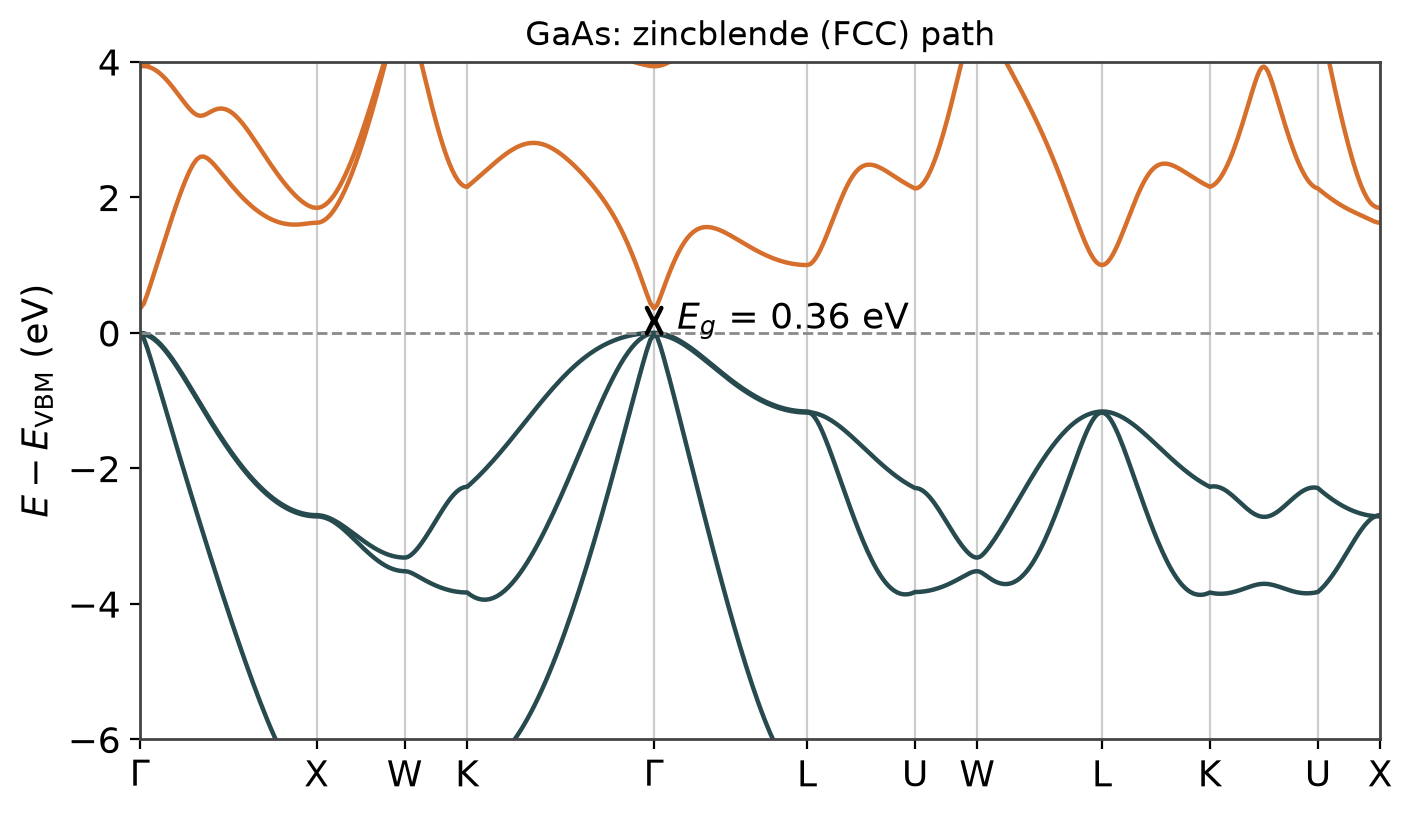
\includegraphics[width=\textwidth]{figures/gaas_bands.png}
			\par\vspace{0.05cm}
			{\footnotesize
			\begin{tabular}{lcc}
				\toprule
				 & GaAs & h-BN \\
				\midrule
				Gap, path / mesh (eV) & 0.361 / 0.361 & 4.589 / 4.589 \\
				Character & direct ($\Gamma$) & direct (K) \\
				\bottomrule
			\end{tabular}}
			\par\vspace{0.1cm}
			\metroset{block=fill}
			\begin{alertblock}{Choosing the zero: \texttt{--shift}}
				\small
				\texttt{vbm}: semiconductors \quad \texttt{fermi}: metals\\
				\texttt{manual}: common reference across systems
			\end{alertblock}
		\end{column}
	\end{columns}
\end{frame}

%-------------------------------------------------
% SLIDE 2.2.7 - stb-dos
%-------------------------------------------------
\begin{frame}[fragile]{\texttt{stb-dos}: Total, Atom, and Species PDOS}
	\begin{columns}[T]
		\begin{column}{0.44\textwidth}
			\metroset{block=fill}
			\begin{block}{Command}
				\footnotesize
\begin{verbatim}
stb-dos --label siesta \
  --shift vbm --save-report \
  --save-gnuplot
\end{verbatim}
			\end{block}
			\vspace{-0.1cm}
			\begin{block}{Options}
				\small
				\begin{itemize}
					\item \texttt{--type}: \texttt{total}, \texttt{atom}, \texttt{species}
					\item \texttt{--projection}: \texttt{l} (s, p, d), \texttt{ml} ($p_x$, $d_{xy}$, \ldots)
					\item \texttt{--shift vbm}: same zero as \texttt{stb-bands}
				\end{itemize}
			\end{block}
			\vspace{-0.1cm}
			\begin{block}{Outputs (each with a \texttt{.gplot})}
				\small
				\texttt{dos\_total.dat}, \texttt{dos\_per\_atom/}, \texttt{dos\_per\_species/}
			\end{block}
		\end{column}
		\begin{column}{0.54\textwidth}
			\centering
			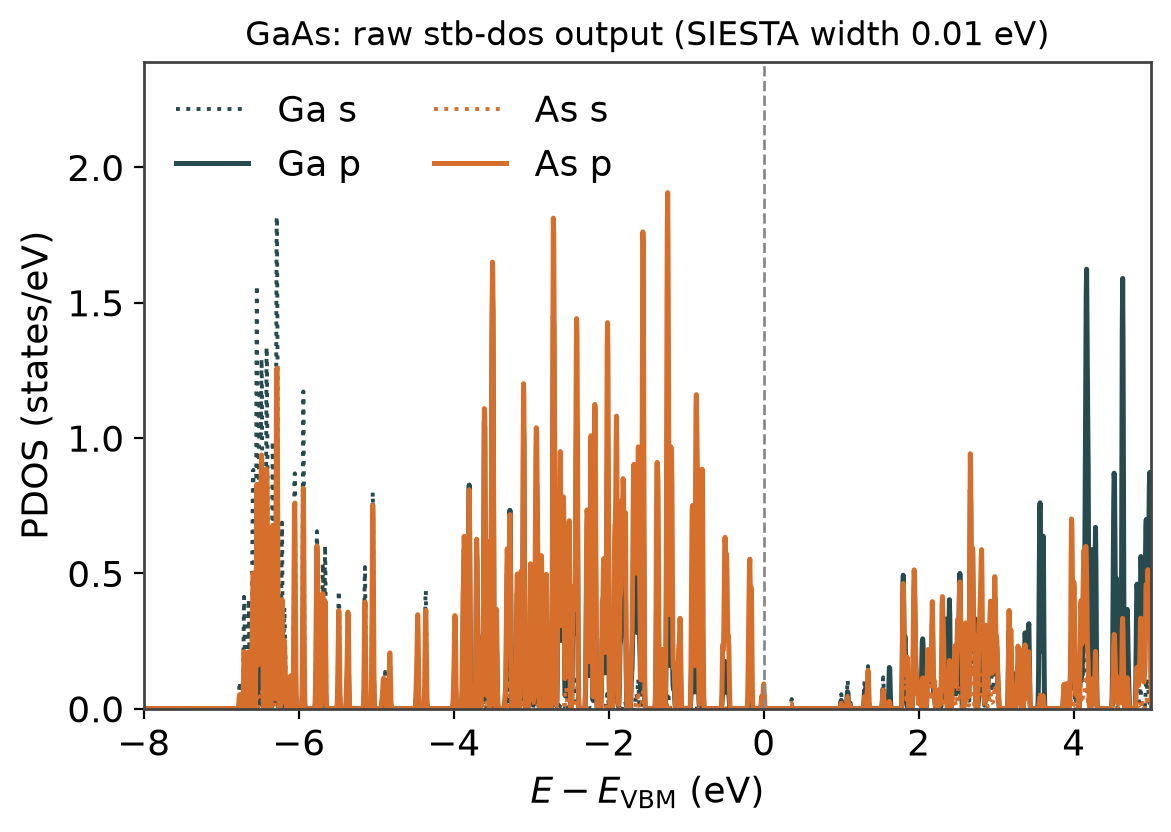
\includegraphics[width=\textwidth]{figures/gaas_pdos.png}
			\par\vspace{0.1cm}
			\metroset{block=fill}
			\begin{alertblock}{Spiky is not wrong}
				\small
				\begin{itemize}
					\item 0.01~eV peak width: each k point shows
					\item Smooth it with \texttt{stb-convdos} (2.3)
				\end{itemize}
			\end{alertblock}
		\end{column}
	\end{columns}
\end{frame}

%%%%%%%%%%%%%%%%%%%%%%%%%%%%%%%%%%%%%%%%%%%%%%%%%%%%%%%%
\section{Hands-on: Bands and DOS of GaAs and h-BN}
%%%%%%%%%%%%%%%%%%%%%%%%%%%%%%%%%%%%%%%%%%%%%%%%%%%%%%%%


%%%%%%%%%%%%%%%%%%%%%%%%%%%%%%%%%%%%%%%%%%%%%%%%%%%%%%%%
\section{Critical Reading of Electronic Results}
%%%%%%%%%%%%%%%%%%%%%%%%%%%%%%%%%%%%%%%%%%%%%%%%%%%%%%%%

%-------------------------------------------------
% SLIDE 2.3.1 - Theory: broadening
%-------------------------------------------------
\begin{frame}{Broadening: Resolution, Not Accuracy}
	\begin{columns}[T]
		\begin{column}{0.42\textwidth}
			\metroset{block=fill}
			\begin{block}{Gaussian convolution}
				\[
					\tilde g(E) = \int g(E')\,
					\frac{e^{-(E-E')^2/2\sigma^2}}{\sigma\sqrt{2\pi}}\,dE'
				\]
				{\scriptsize $\mathrm{FWHM} = 2.3548\,\sigma$. The kernel has unit area,
				so the number of states is conserved.}
			\end{block}
			\vspace{0.05cm}
			\begin{block}{Why the raw DOS is spiky}
				A finite k mesh gives a finite set of $\varepsilon_{n\mathbf{k}}$.
				A narrow peak shows each one; a wider one interpolates between them.
			\end{block}
		\end{column}
		\begin{column}{0.56\textwidth}
			\centering
			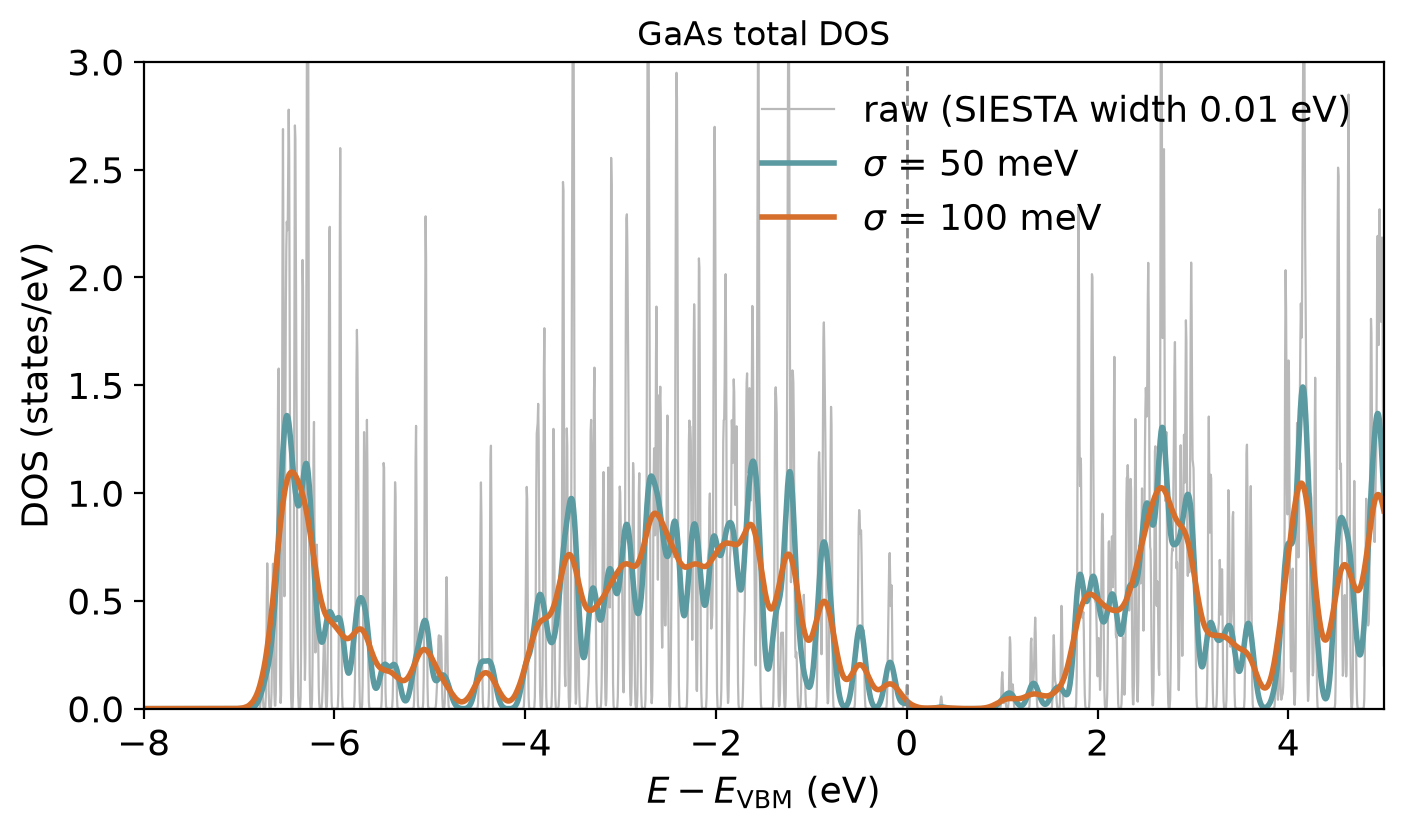
\includegraphics[width=\textwidth]{figures/gaas_convdos.png}
			\par\vspace{0.05cm}
			{\small Same SIESTA run, three widths.}
		\end{column}
	\end{columns}
	\vspace{0.15cm}
	\metroset{block=fill}
	\begin{alertblock}{A smoother curve is not a better calculation}
		\small
		\begin{itemize}
			\item $\sigma$ is a display choice: state it in every figure
			\item Too wide merges peaks and smears the band edges into the gap
			\item Only a denser k mesh adds information
		\end{itemize}
	\end{alertblock}
\end{frame}

%-------------------------------------------------
% SLIDE 2.3.2 - Theory: work function
%-------------------------------------------------
\begin{frame}{Work Function and the Vacuum Level}
	\begin{columns}[T]
		\begin{column}{0.42\textwidth}
			\metroset{block=fill}
			\begin{block}{Definition}
				\[
					\Phi = E_{\text{vac}} - E_F
				\]
				\[
					\bar V(z) = \frac{1}{A}\iint_A V(x,y,z)\,dx\,dy
				\]
				{\scriptsize $E_{\text{vac}}$ is the flat plateau of the planar-averaged
				total potential $\bar V(z)$ far from the layer.}
			\end{block}
			\vspace{0.05cm}
			\begin{block}{Requirements}
				\small
				\begin{itemize}
					\item A vacuum region wide enough to flatten $\bar V$
					\item Dipole correction for asymmetric slabs
					\item \textbf{Not defined} for a periodic 3D crystal (GaAs)
				\end{itemize}
			\end{block}
		\end{column}
		\begin{column}{0.56\textwidth}
			\centering
			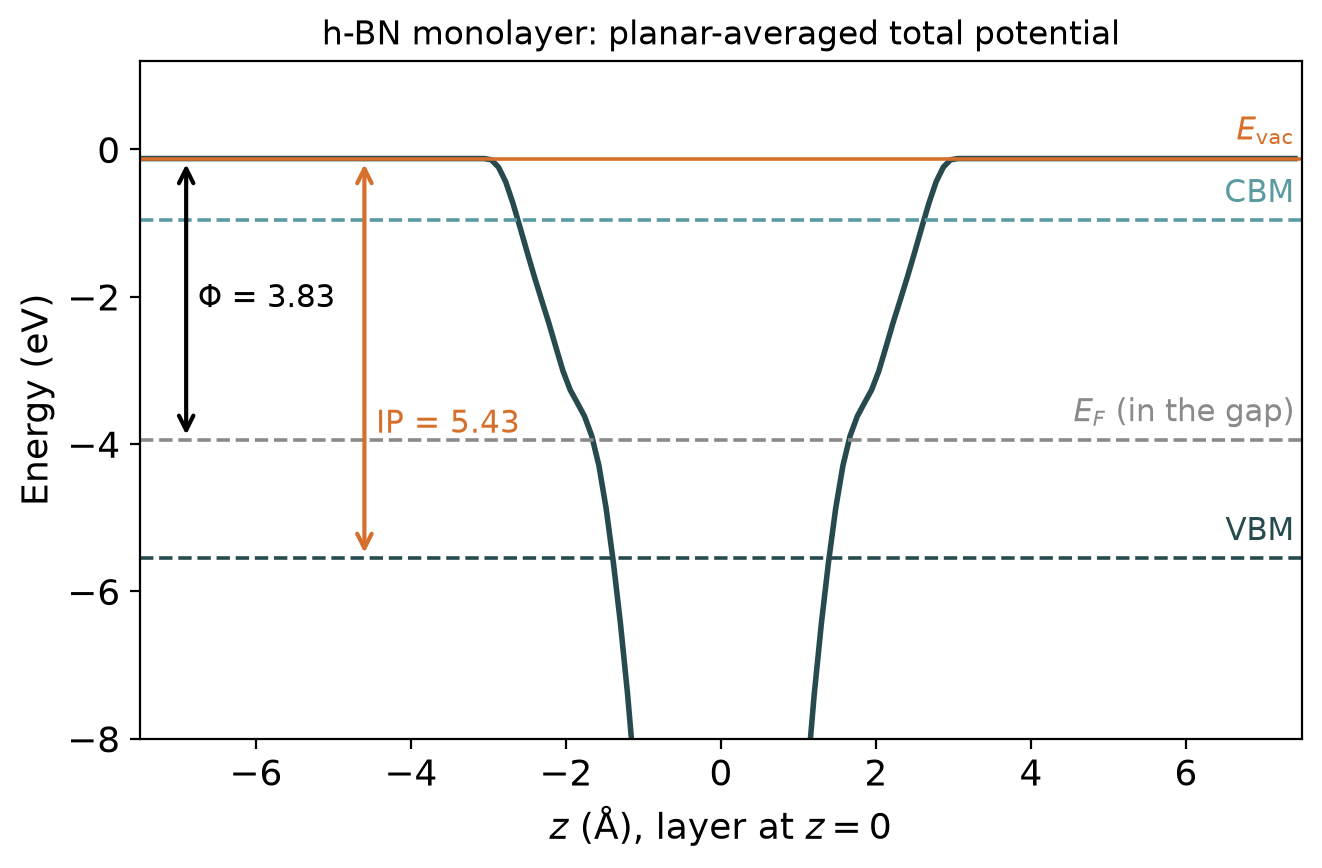
\includegraphics[width=\textwidth]{figures/hbn_workfunction.png}
		\end{column}
	\end{columns}
	\vspace{0.15cm}
	\metroset{block=fill}
	\begin{alertblock}{Insulators: $E_F$ floats in the gap}
		\small
		\begin{itemize}
			\item In h-BN, $E_F$ sits mid-gap and moves with smearing
			\item Report band-edge quantities:
				IP $= E_{\text{vac}} - E_{\text{VBM}} = 5.43$~eV, \;
				EA $= E_{\text{vac}} - E_{\text{CBM}} = 0.84$~eV
		\end{itemize}
	\end{alertblock}
\end{frame}

%-------------------------------------------------
% SLIDE 2.3.3 - Theory: fatbands
%-------------------------------------------------
\begin{frame}{Orbital Character Along the Bands: Fatbands}
	\begin{columns}[T]
		\begin{column}{0.42\textwidth}
			\metroset{block=fill}
			\begin{block}{Weight of orbital $\mu$ in state $n\mathbf{k}$}
				\[
					w_{\mu,n\mathbf{k}} = \mathrm{Re}\!\left[c^{*}_{\mu,n\mathbf{k}}\,
					(\mathbf{S}\,\mathbf{c}_{n\mathbf{k}})_\mu\right]
				\]
				\[
					\sum_\mu w_{\mu,n\mathbf{k}} = 1
				\]
				{\scriptsize Marker size $\propto w$. Summing $w\,\delta(E-\varepsilon_{n\mathbf{k}})$
				over the whole BZ gives the PDOS.}
			\end{block}
			\vspace{0.05cm}
			\begin{block}{PDOS vs fatbands}
				PDOS: \emph{which energies}.\\
				Fatbands: \emph{which energies and which $\mathbf{k}$}.
			\end{block}
		\end{column}
		\begin{column}{0.56\textwidth}
			\centering
			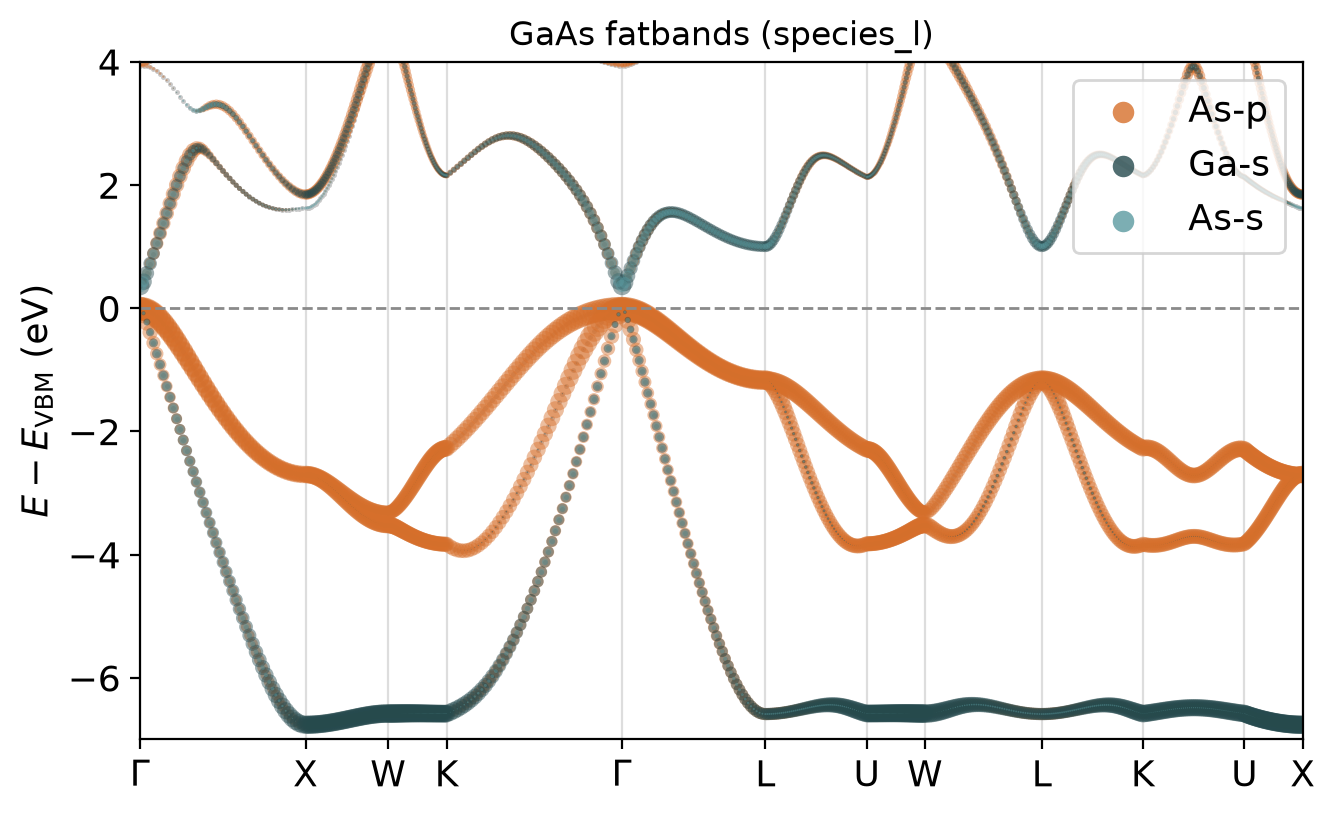
\includegraphics[width=\textwidth]{figures/gaas_fatbands.png}
			\par\vspace{0.05cm}
			{\small GaAs: VBM is As-$p$; CBM at $\Gamma$ is Ga-$s$/As-$s$.}
		\end{column}
	\end{columns}
	\vspace{0.15cm}
	\metroset{block=fill}
	\begin{alertblock}{A projection, not a measurement}
		\small
		\begin{itemize}
			\item Mulliken-type weights depend on the basis
			\item Non-orthogonal basis: a weight can be slightly $<0$ or $>1$
			\item Compare trends, not decimals
		\end{itemize}
	\end{alertblock}
\end{frame}

%-------------------------------------------------
% SLIDE 2.3.4 - How to do it in STB
%-------------------------------------------------
\begin{frame}{Three Readings, Three Requirements}
	\centering
	\resizebox{1.0\textwidth}{!}{%
	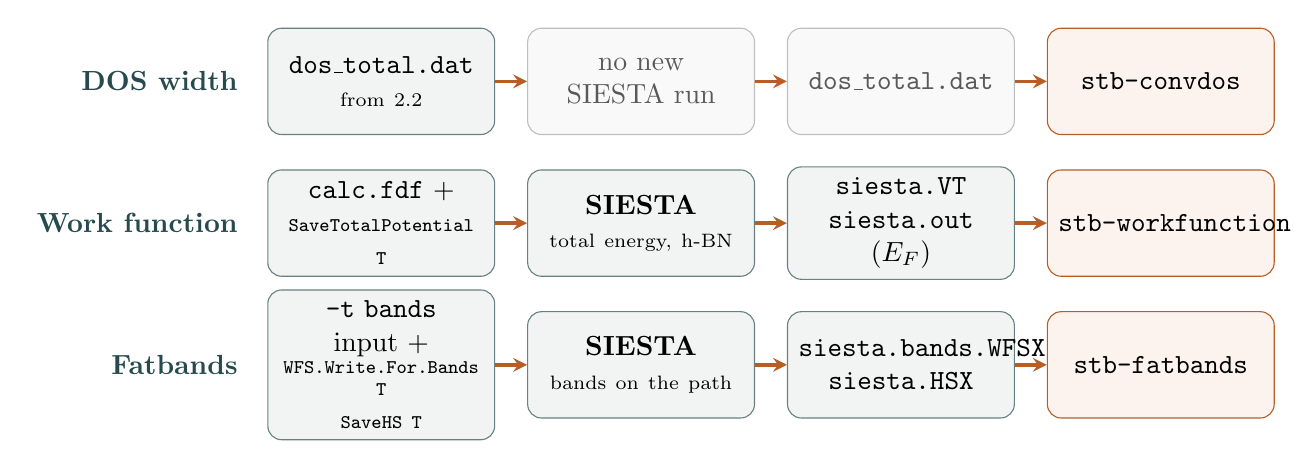
\begin{tikzpicture}[
		stage/.style={
			draw=stbteal!70,fill=stbteal!6,rounded corners=5pt,
			text width=2.6cm,minimum height=1.35cm,align=center,inner sep=4pt
		},
		tool/.style={stage,draw=stborange!85!black,fill=stborange!8},
		none/.style={stage,draw=gray!50,fill=gray!5,text=gray!70!black},
		flow/.style={->,>=stealth,line width=1.2pt,draw=stborange!85!black},
		row/.style={font=\bfseries\color{stbteal},anchor=east}
	]
		% row 1
		\node[row] at (-1.7,0) {DOS width};
		\node[stage] (a1) at (0,0) {\texttt{dos\_total.dat}\\{\scriptsize from 2.2}};
		\node[none] (a2) at (3.3,0) {no new SIESTA run};
		\node[none] (a3) at (6.6,0) {\texttt{dos\_total.dat}};
		\node[tool] (a4) at (9.9,0) {\texttt{stb-convdos}};
		% row 2
		\node[row] at (-1.7,-1.8) {Work function};
		\node[stage] (b1) at (0,-1.8) {\texttt{calc.fdf} +\\{\scriptsize\texttt{SaveTotalPotential T}}};
		\node[stage] (b2) at (3.3,-1.8) {\textbf{SIESTA}\\{\scriptsize total energy, h-BN}};
		\node[stage] (b3) at (6.6,-1.8) {\texttt{siesta.VT}\\\texttt{siesta.out} ($E_F$)};
		\node[tool] (b4) at (9.9,-1.8) {\texttt{stb-workfunction}};
		% row 3
		\node[row] at (-1.7,-3.6) {Fatbands};
		\node[stage] (c1) at (0,-3.6) {\texttt{-t bands} input +\\{\scriptsize\texttt{WFS.Write.For.Bands T}\\\texttt{SaveHS T}}};
		\node[stage] (c2) at (3.3,-3.6) {\textbf{SIESTA}\\{\scriptsize bands on the path}};
		\node[stage] (c3) at (6.6,-3.6) {\texttt{siesta.bands.WFSX}\\\texttt{siesta.HSX}};
		\node[tool] (c4) at (9.9,-3.6) {\texttt{stb-fatbands}};
		\foreach \r in {a,b,c}{
			\draw[flow] (\r1) -- (\r2); \draw[flow] (\r2) -- (\r3); \draw[flow] (\r3) -- (\r4);
		}
	\end{tikzpicture}%
	}
	\vspace{0.3cm}
	\metroset{block=fill}
	\begin{alertblock}{SIESTA only writes what you ask for}
		\small
		\begin{itemize}
			\item \texttt{.VT}, \texttt{.WFSX}, \texttt{.HSX} are off by default: set the flag \emph{before} the run
			\item A small wrapper \texttt{.fdf} that \texttt{\%include}s \texttt{calc.fdf} keeps the template untouched
		\end{itemize}
	\end{alertblock}
\end{frame}

%-------------------------------------------------
% SLIDE 2.3.5 - stb-convdos
%-------------------------------------------------
\begin{frame}[fragile]{\texttt{stb-convdos}: Gaussian Broadening}
	\begin{columns}[T]
		\begin{column}{0.50\textwidth}
			{\scriptsize
\begin{verbatim}
stb-convdos --file dos_total.dat --sigma 50 \
  --out dos_total_50meV.dat --no-plot --save-report
\end{verbatim}
			}
			\metroset{block=fill}
			\begin{block}{Options}
				\begin{itemize}
					\item \texttt{--sigma} or \texttt{--fwhm}, in meV
					\item \texttt{--dir}: broaden a whole \texttt{stb-dos} output tree
					\item \texttt{--size}: kernel width in samples (default $\pm3\sigma$)
					\item Every DOS column is broadened; the energy grid is kept
				\end{itemize}
			\end{block}
		\end{column}
		\begin{column}{0.46\textwidth}
			\metroset{block=fill}
			\begin{block}{GaAs report, $\sigma = 50$~meV}
				\ttfamily\scriptsize
				Grid spacing : 0.005 eV\\
				Sigma \ \ \ \ \ \ \ : 50 meV (10 samples)\\
				Kernel size \ : 61 samples\\[4pt]
				\normalfont\textbf{Conservation check}\\[2pt]
				\begin{tabular}{lrr}
					\toprule
					Column & Before & After \\
					\midrule
					s & 1.8251 & 1.8250 \\
					p & 7.5399 & 7.5311 \\
					d & 10.8686 & 10.8667 \\
					\bottomrule
				\end{tabular}
			\end{block}
		\end{column}
	\end{columns}
	\vspace{0.2cm}
	\metroset{block=fill}
	\begin{alertblock}{Read the conservation check}
		\small
		\begin{itemize}
			\item Drift above a few tenths of a percent: weight leaked off the energy window
			\item Fix: widen the PDOS window in SIESTA, or reduce $\sigma$
		\end{itemize}
	\end{alertblock}
\end{frame}

%-------------------------------------------------
% SLIDE 2.3.6 - stb-workfunction
%-------------------------------------------------
\begin{frame}[fragile]{\texttt{stb-workfunction}: Vacuum Level from \texttt{.VT}}
	\begin{columns}[T]
		\begin{column}{0.50\textwidth}
			{\scriptsize
\begin{verbatim}
stb-workfunction --label siesta \
  --save-report --save-gnuplot
\end{verbatim}
			}
			\metroset{block=fill}
			\begin{block}{What it does}
				\begin{itemize}
					\item Detects the vacuum axis from the structure
					\item Averages \texttt{.VT} over the plane; finds flat plateaus
					\item Asymmetric slab: reports \textbf{two} work functions
					\item Warns if the plateau has a slope (missing dipole correction)
				\end{itemize}
			\end{block}
		\end{column}
		\begin{column}{0.46\textwidth}
			\metroset{block=fill}
			\begin{block}{h-BN report}
				\ttfamily\scriptsize
				E\_F \ \ \ \ \ \ \ \ \ : -3.9494 eV (siesta.out)\\
				Axis \ \ \ \ \ \ \ \ : 2 (z), auto-detected\\
				Plateau std : 0.000014 eV (flat)\\[3pt]
				Vacuum level: -0.1240 eV\\
				\textcolor{stborange!85!black}{\textbf{Work function: 3.8254 eV}}
			\end{block}
			\vspace{0.1cm}
			\begin{alertblock}{Check before quoting}
				Flat plateau? Symmetric slab? Metal or insulator?
				For h-BN, quote IP = 5.43~eV next to $\Phi$.
			\end{alertblock}
		\end{column}
	\end{columns}
	\vspace{0.15cm}
	{\scriptsize Do not run it on GaAs: a fully periodic 3D cell has no vacuum, so there is no $E_{\text{vac}}$.}
\end{frame}

%-------------------------------------------------
% SLIDE 2.3.7 - stb-fatbands
%-------------------------------------------------
\begin{frame}[fragile]{\texttt{stb-fatbands}: Orbital-Projected Bands}
	\begin{columns}[T]
		\begin{column}{0.44\textwidth}
			{\scriptsize
\begin{verbatim}
stb-fatbands --label siesta --shift vbm \
  --projection species_l \
  --save-report --save-gnuplot
\end{verbatim}
			}
			\metroset{block=fill}
			\begin{block}{Projections}
				\texttt{l}, \texttt{ml}, \texttt{atom}, \texttt{species},
				\texttt{species\_l} (e.g.\ \texttt{N-p}, \texttt{B-s});
				\texttt{--category} keeps only some
			\end{block}
			\begin{block}{Built-in checks}
				\begin{itemize}
					\item \texttt{.bands} and \texttt{.WFSX} cross-checked at sampled k points
					\item With \texttt{.HSX}: overlap-weighted (accurate) weights
					\item Without it: falls back to the \texttt{.fdf}, with a warning
				\end{itemize}
			\end{block}
		\end{column}
		\begin{column}{0.54\textwidth}
			\centering
			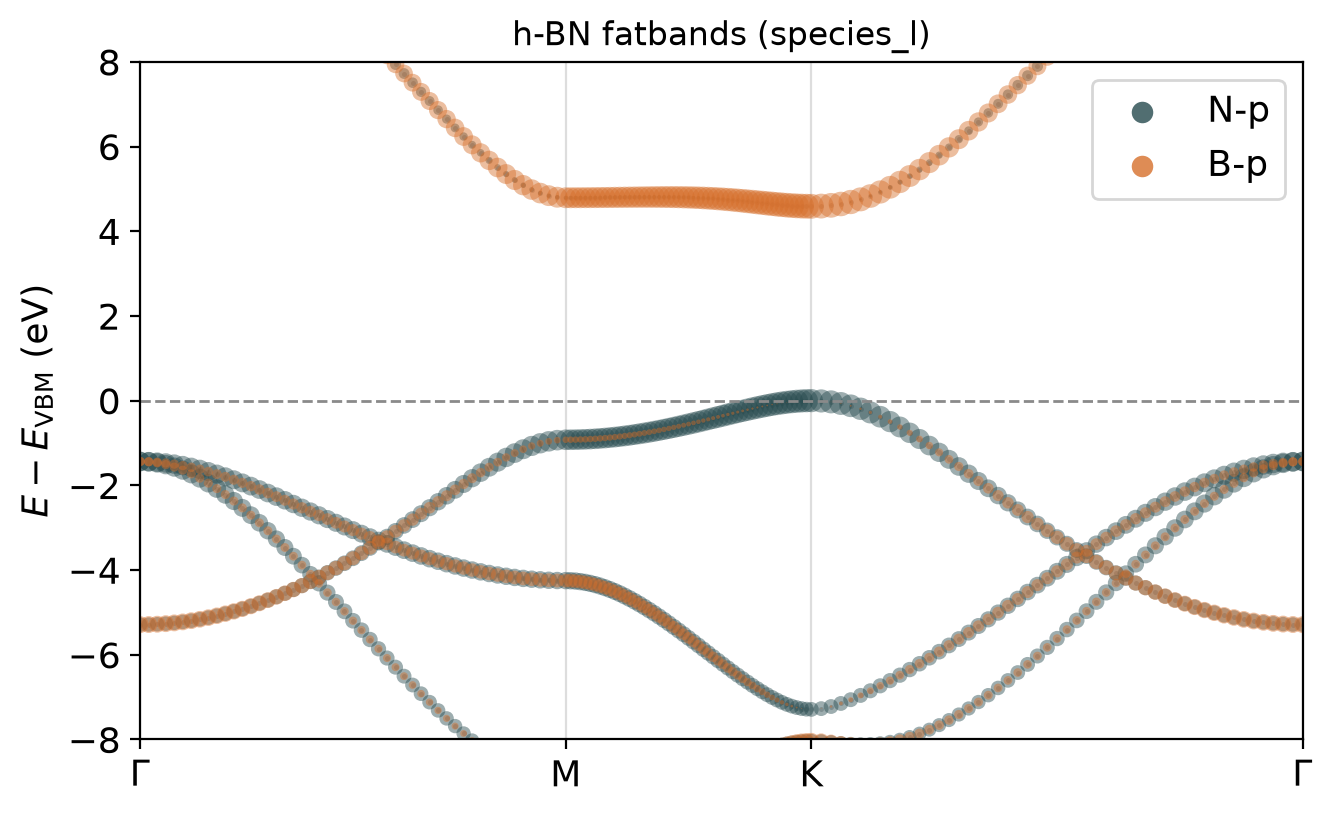
\includegraphics[width=\textwidth]{figures/hbn_fatbands.png}
			\par\vspace{0.1cm}
			\metroset{block=fill}
			\begin{alertblock}{h-BN}
				\small
				\begin{itemize}
					\item At K: valence N-$p$, conduction B-$p$
					\item Same picture as the PDOS, now resolved in $\mathbf{k}$
				\end{itemize}
			\end{alertblock}
		\end{column}
	\end{columns}
\end{frame}

%%%%%%%%%%%%%%%%%%%%%%%%%%%%%%%%%%%%%%%%%%%%%%%%%%%%%%%%
\section{Hands-on: Broadening, Work Function, and Fatbands}
%%%%%%%%%%%%%%%%%%%%%%%%%%%%%%%%%%%%%%%%%%%%%%%%%%%%%%%%


%%%%%%%%%%%%%%%%%%%%%%%%%%%%%%%%%%%%%%%%%%%%%%%%%%%%%%%%
\section{Adsorption on h-BN}
%%%%%%%%%%%%%%%%%%%%%%%%%%%%%%%%%%%%%%%%%%%%%%%%%%%%%%%%

%-------------------------------------------------
% SLIDE 2.5.1 - Theory: adsorption energy
%-------------------------------------------------
\begin{frame}{Adsorption Energy: Three Calculations, One Number}
	\centering
	\resizebox{0.95\textwidth}{!}{%
	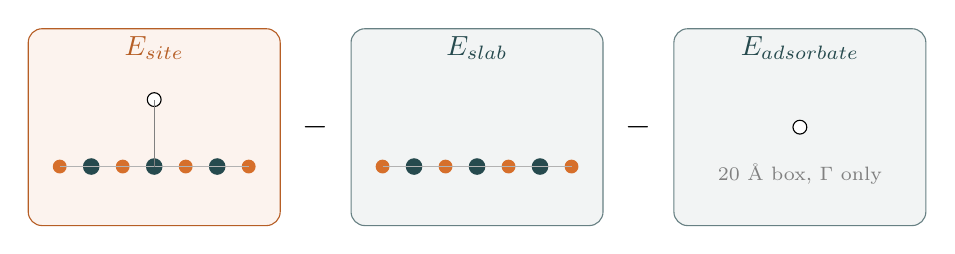
\begin{tikzpicture}[
		box/.style={draw=stbteal!70,fill=stbteal!6,rounded corners=5pt,
			minimum width=3.2cm,minimum height=2.5cm,align=center,inner sep=5pt},
		site/.style={box,draw=stborange!85!black,fill=stborange!8},
		b/.style={circle,fill=stborange,inner sep=0pt,minimum size=5pt},
		n/.style={circle,fill=stbteal,inner sep=0pt,minimum size=6pt},
		h/.style={circle,fill=white,draw=black,inner sep=0pt,minimum size=5pt}
	]
		\node[site] (s) at (0,0) {};
		\hbnlayer{0}{-0.5}
		\node[h] at (0,0.35) {};
		\draw[gray] (0,-0.5) -- (0,0.35);
		\node[font=\bfseries\color{stborange!85!black}] at (0,1.0) {$E_{\text{site}}$};
		\node[font=\large] at (2.05,0) {$-$};
		\node[box] (c) at (4.1,0) {};
		\hbnlayer{4.1}{-0.5}
		\node[font=\bfseries\color{stbteal}] at (4.1,1.0) {$E_{\text{slab}}$};
		\node[font=\large] at (6.15,0) {$-$};
		\node[box] (a) at (8.2,0) {};
		\node[h] at (8.2,0.0) {};
		\node[font=\scriptsize,text=gray] at (8.2,-0.6) {20~\AA\ box, $\Gamma$ only};
		\node[font=\bfseries\color{stbteal}] at (8.2,1.0) {$E_{\text{adsorbate}}$};
	\end{tikzpicture}%
	}
	\[
		E_{\text{ads}} = E_{\text{site}} - E_{\text{slab}} - E_{\text{adsorbate}}
		\qquad (E_{\text{ads}} < 0 \Rightarrow \text{favorable})
	\]
	\begin{columns}[T]
		\begin{column}{0.48\textwidth}
			\metroset{block=fill}
			\begin{block}{Same settings everywhere}
				Basis, mesh, functional, D3, and pseudopotentials must match;
				otherwise the subtraction does not cancel numerical errors.
			\end{block}
		\end{column}
		\begin{column}{0.48\textwidth}
			\metroset{block=fill}
			\begin{block}{Which reference for H?}
				Atomic H measures the bond to the surface.
				$\tfrac{1}{2}E_{\text{H}_2}$ asks whether H prefers the surface or H$_2$
				(H$_2$ binding: 4.5~eV, about 2.2~eV per H).
			\end{block}
		\end{column}
	\end{columns}
\end{frame}

%-------------------------------------------------
% SLIDE 2.5.2 - Theory: physisorption vs chemisorption
%-------------------------------------------------
\begin{frame}{Physisorption or Chemisorption?}
	\begin{columns}[T]
		\begin{column}{0.56\textwidth}
			\centering
			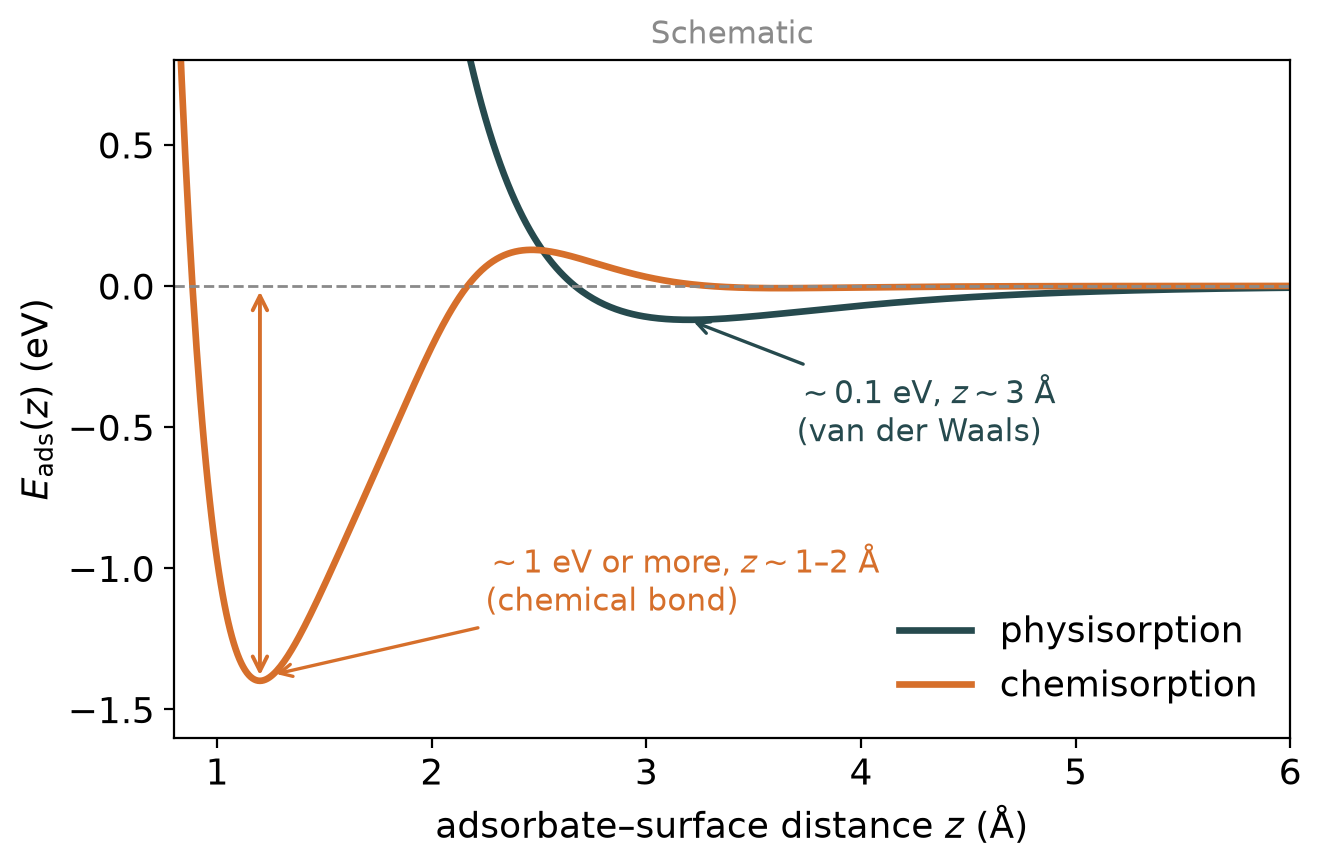
\includegraphics[width=\textwidth]{figures/adsorption_pes.png}
		\end{column}
		\begin{column}{0.42\textwidth}
			\metroset{block=fill}
			\begin{block}{Physisorption}
				Dispersion only; electronic structure barely changes.
				Weak, long distance: needs D3.
			\end{block}
			\begin{block}{Chemisorption}
				A bond forms: charge transfer, rehybridization, possible barrier.
				On h-BN, H on top of B or N pulls the atom out of plane
				($sp^2 \rightarrow sp^3$-like).
			\end{block}
		\end{column}
	\end{columns}
	\vspace{0.2cm}
	\metroset{block=fill}
	\begin{alertblock}{The start height decides which well you find}
		\small
		\begin{itemize}
			\item A relaxation only goes downhill: 1.5~\AA\ targets the chemical well, a high start can end in the shallow one
			\item Check the final $z$ and the bonds
		\end{itemize}
	\end{alertblock}
\end{frame}

%-------------------------------------------------
% SLIDE 2.5.3 - Theory: supercell, coverage, vacuum
%-------------------------------------------------
\begin{frame}{Supercell, Coverage, and Vacuum}
	\centering
	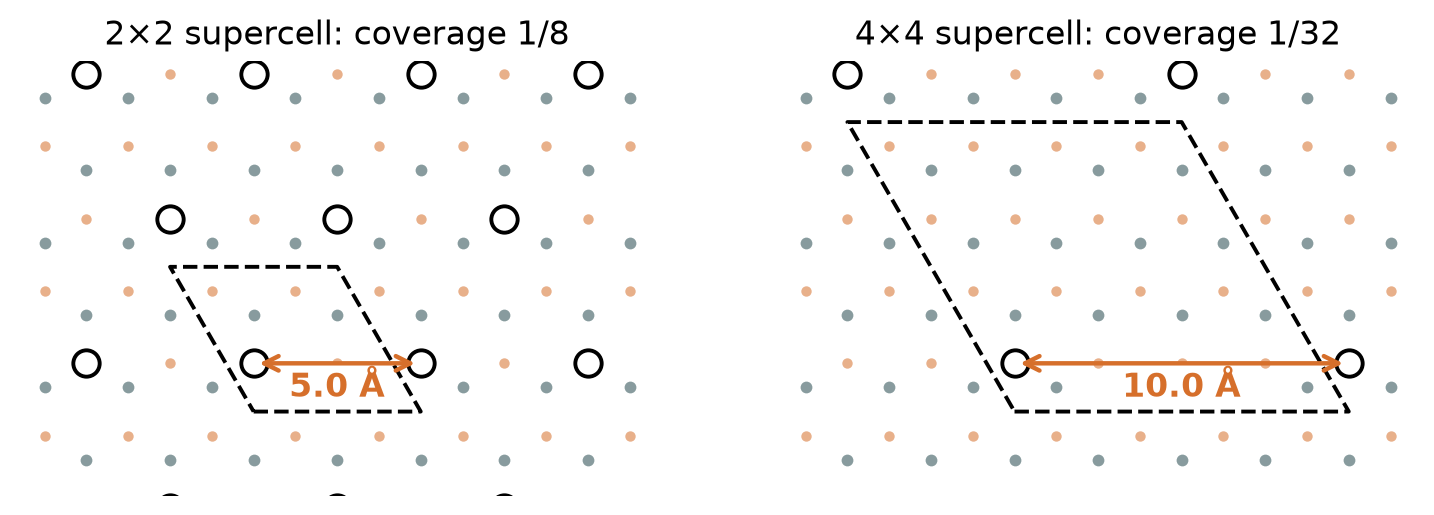
\includegraphics[width=0.82\textwidth]{figures/adsorption_supercell.png}
	\par\vspace{0.1cm}
	\begin{columns}[T]
		\begin{column}{0.32\textwidth}
			\metroset{block=fill}
			\begin{block}{In-plane}
				Periodic images interact. Bigger cell $\rightarrow$ lower coverage,
				closer to an isolated adsorbate.
			\end{block}
		\end{column}
		\begin{column}{0.32\textwidth}
			\metroset{block=fill}
			\begin{block}{Out-of-plane}
				15~\AA\ cell: enough vacuum for the potential to flatten.
				Dipole correction removes the artificial field.
			\end{block}
		\end{column}
		\begin{column}{0.32\textwidth}
			\metroset{block=fill}
			\begin{block}{k points}
				A 4$\times$4 cell needs 4$\times$ fewer k per direction:
				$3{\times}3{\times}1$ here $\approx 12{\times}12$ in the primitive cell.
			\end{block}
		\end{column}
	\end{columns}
\end{frame}

%-------------------------------------------------
% SLIDE 2.5.4 - Theory: BSSE in adsorption
%-------------------------------------------------
\begin{frame}{Basis-Set Superposition Error in Adsorption}
	\begin{columns}[T]
		\begin{column}{0.48\textwidth}
			\metroset{block=fill}
			\begin{block}{Why LCAO over-binds}
				In the site calculation, H can borrow the slab's orbitals (and vice versa).
				Each fragment is described better \emph{together} than \emph{alone},
				so $E_{\text{ads}}$ comes out too negative.
			\end{block}
			\vspace{0.05cm}
			\begin{block}{Counterpoise (Boys--Bernardi)}
				\[
					E_{\text{ads}}^{\text{CP}} = E_{\text{ads}} + \delta_{\text{slab}} + \delta_{\text{H}}
				\]
				\[
					\delta_X = E_X - E_X^{\,[\text{ghost}]} > 0
				\]
				{\scriptsize Ghost = orbitals without nucleus or electrons. Both terms of
				$\delta_X$ use fragment $X$ at the \textbf{relaxed site geometry}.}
			\end{block}
		\end{column}
		\begin{column}{0.48\textwidth}
			\centering
			\resizebox{\textwidth}{!}{%
			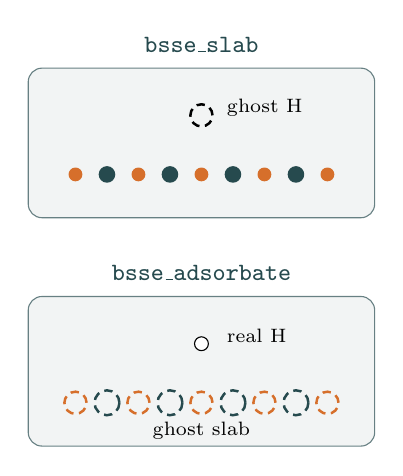
\begin{tikzpicture}[
				box/.style={draw=stbteal!70,fill=stbteal!6,rounded corners=5pt,
					minimum width=4.4cm,minimum height=1.9cm},
				b/.style={circle,fill=stborange,inner sep=0pt,minimum size=5pt},
				n/.style={circle,fill=stbteal,inner sep=0pt,minimum size=6pt},
				gb/.style={circle,draw=stborange,densely dashed,line width=0.9pt,inner sep=0pt,minimum size=8pt},
				gn/.style={circle,draw=stbteal,densely dashed,line width=0.9pt,inner sep=0pt,minimum size=9pt},
				h/.style={circle,fill=white,draw=black,inner sep=0pt,minimum size=5pt},
				gh/.style={circle,draw=black,densely dashed,line width=0.9pt,inner sep=0pt,minimum size=8pt}
			]
				\node[box] at (0,0) {};
				\foreach \i in {0,...,8}{\pgfmathsetmacro{\xx}{-1.6+0.4*\i}
					\ifodd\i \node[n] at (\xx,-0.4) {}; \else \node[b] at (\xx,-0.4) {}; \fi}
				\node[gh] at (0,0.35) {};
				\node[font=\scriptsize,anchor=west] at (0.2,0.45) {ghost H};
				\node[font=\bfseries\small\color{stbteal}] at (0,1.25) {\texttt{bsse\_slab}};
				\node[box] at (0,-2.9) {};
				\foreach \i in {0,...,8}{\pgfmathsetmacro{\xx}{-1.6+0.4*\i}
					\ifodd\i \node[gn] at (\xx,-3.3) {}; \else \node[gb] at (\xx,-3.3) {}; \fi}
				\node[h] at (0,-2.55) {};
				\node[font=\scriptsize,anchor=west] at (0.2,-2.45) {real H};
				\node[font=\scriptsize] at (0,-3.65) {ghost slab};
				\node[font=\bfseries\small\color{stbteal}] at (0,-1.65) {\texttt{bsse\_adsorbate}};
			\end{tikzpicture}%
			}
		\end{column}
	\end{columns}
	\vspace{0.0cm}
	\metroset{block=fill}
	\begin{alertblock}{Same correction you saw for cohesive energy}
		\small
		\begin{itemize}
			\item Part 1: BSSE moved $E_{\text{coh}}$ of GaAs by $\sim$1~eV/atom
			\item Adsorption: it can change the ranking of close sites
		\end{itemize}
	\end{alertblock}
\end{frame}

%-------------------------------------------------
% SLIDE 2.5.5 - Theory: physics settings
%-------------------------------------------------
\begin{frame}{Getting the Physics Right Before the Numbers}
	\centering
	\resizebox{0.98\textwidth}{!}{%
	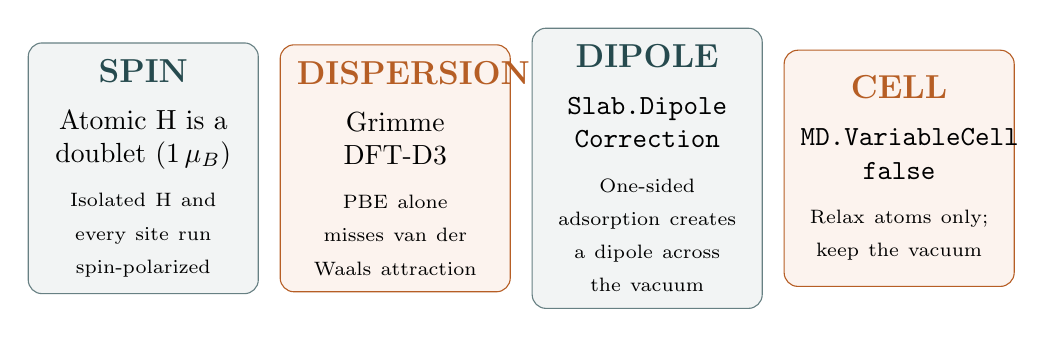
\begin{tikzpicture}[
		card/.style={draw=stbteal!70,fill=stbteal!6,rounded corners=5pt,
			text width=2.5cm,minimum height=3.0cm,align=center,inner sep=6pt},
		alt/.style={card,draw=stborange!85!black,fill=stborange!8}
	]
		\node[card] at (0,0) {
			{\color{stbteal}\large\bfseries SPIN}\\[5pt]
			Atomic H is a doublet ($1\,\mu_B$)\\[4pt]
			{\scriptsize Isolated H and every site run spin-polarized}
		};
		\node[alt] at (3.2,0) {
			{\color{stborange!85!black}\large\bfseries DISPERSION}\\[5pt]
			Grimme DFT-D3\\[4pt]
			{\scriptsize PBE alone misses van der Waals attraction}
		};
		\node[card] at (6.4,0) {
			{\color{stbteal}\large\bfseries DIPOLE}\\[5pt]
			\texttt{Slab.Dipole}\\\texttt{Correction}\\[4pt]
			{\scriptsize One-sided adsorption creates a dipole across the vacuum}
		};
		\node[alt] at (9.6,0) {
			{\color{stborange!85!black}\large\bfseries CELL}\\[5pt]
			\texttt{MD.VariableCell}\\\texttt{false}\\[4pt]
			{\scriptsize Relax atoms only; keep the vacuum}
		};
	\end{tikzpicture}%
	}
	\vspace{0.3cm}
	\begin{columns}[T]
		\begin{column}{0.48\textwidth}
			\metroset{block=fill}
			\begin{block}{Sites are starting points}
				\emph{ontop}, \emph{bridge}, and \emph{hollow} label where the adsorbate
				\emph{starts}. The relaxation may move it elsewhere: always inspect the final geometry.
			\end{block}
		\end{column}
		\begin{column}{0.48\textwidth}
			\metroset{block=fill}
			\begin{alertblock}{First occurrence wins}
				\small
				\begin{itemize}
					\item SIESTA reads the \emph{first} value of each label
					\item STB puts these settings in \texttt{config\_extra.fdf}, included at the \textbf{top} of \texttt{calc.fdf}
				\end{itemize}
			\end{alertblock}
		\end{column}
	\end{columns}
\end{frame}


%-------------------------------------------------
% SLIDE 2.5.5b - Theory: Gibbs free energy of adsorption
%-------------------------------------------------
\begin{frame}{Beyond $E_{\text{ads}}$: Gibbs Free Energy of Adsorption}
	\begin{columns}[T]
		\begin{column}{0.40\textwidth}
			\metroset{block=fill}
			\begin{block}{Add vibrations and entropy}
				\[
					\Delta G(T) = \underbrace{E_{\text{ads}} + \Delta\mathrm{ZPE}}_{D_0} - T\,\Delta S
				\]
				{\scriptsize $\mathrm{ZPE} = \sum_i \tfrac{1}{2}\hbar\omega_i$, $\omega_i$ from a finite-difference Hessian (harmonic approximation).
				$\Delta X = X_{\text{site}} - X_{\text{reference}}$.}
			\end{block}
			\vspace{0.05cm}
			\begin{block}{H on h-BN}
				\small
				\begin{itemize}
					\item \textbf{Site}: 3 H modes (1 stretch, 2 bends), substrate frozen
					\item \textbf{Reference}: free H, no vibrations, but translational entropy (ideal gas, 1~bar)
				\end{itemize}
			\end{block}
		\end{column}
		\begin{column}{0.58\textwidth}
			\centering
			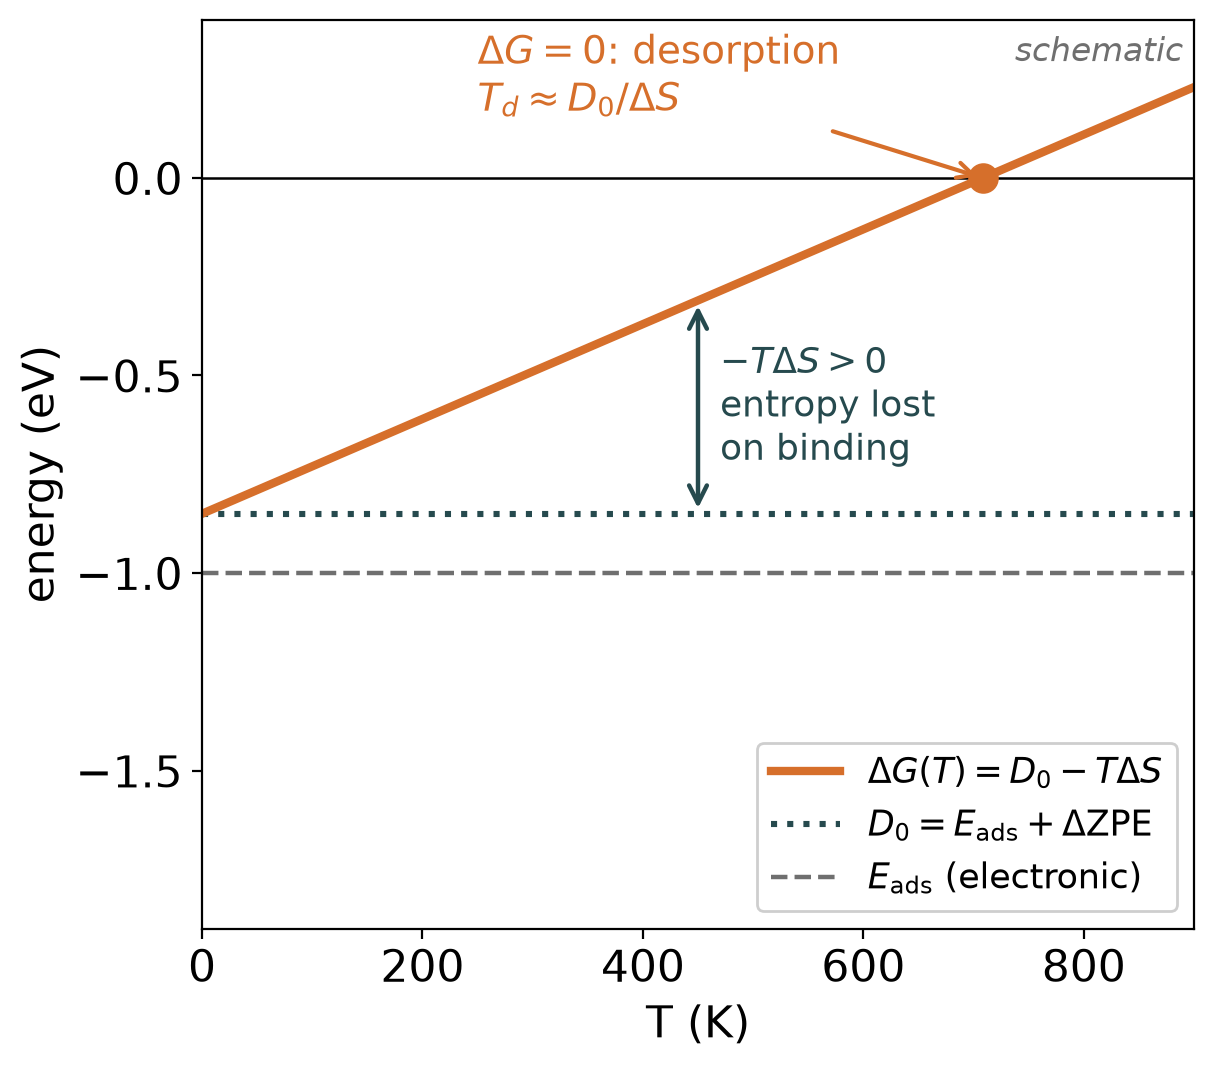
\includegraphics[width=\textwidth,height=0.66\textheight,keepaspectratio]{figures/adsorption_gibbs_schematic.png}
		\end{column}
	\end{columns}
	\vspace{0.0cm}
	\metroset{block=fill}
	\begin{alertblock}{Binding costs entropy}
		\small
		\begin{itemize}
			\item The adsorbate loses freedom: $\Delta S < 0$, so $\Delta G$ rises with $T$
			\item $T_d$ is a thermodynamic estimate, not a kinetic prediction
		\end{itemize}
	\end{alertblock}
\end{frame}

%-------------------------------------------------
% SLIDE 2.5.5c - Theory: how Delta S is computed
%-------------------------------------------------
\begin{frame}{How $\Delta S$ Is Computed}
	\[
		\Delta S(T) = S_{\text{site}}(T) - S_{\text{ref}}(T)
	\]
	\begin{columns}[T]
		\begin{column}{0.48\textwidth}
			\metroset{block=fill}
			\begin{block}{Adsorbed H: harmonic oscillators}
				\[
					S_{\text{site}} = k_B \sum_{i=1}^{3}
					\left[\frac{x_i}{e^{x_i}-1} - \ln\!\left(1-e^{-x_i}\right)\right]
				\]
				\[
					x_i = \frac{\hbar\omega_i}{k_B T}
				\]
				{\scriptsize $\omega_i$ from the local Hessian. Stiff modes ($\hbar\omega \gg k_BT$)
				contribute almost nothing.}\\[4pt]
				{\scriptsize
				\begin{tabular}{lccc}
					\toprule
					$\tilde\nu$ (cm$^{-1}$) & 500 & 1000 & 2500 \\
					$S$ at 298 K (J/(mol\,K)) & 2.8 & 0.4 & 0.0 \\
					\bottomrule
				\end{tabular}}
			\end{block}
		\end{column}
		\begin{column}{0.48\textwidth}
			\metroset{block=fill}
			\begin{block}{Free H atom: ideal gas at 1 bar}
				\[
					S_{\text{ref}} = S_{\text{trans}} + S_{\text{rot}} + S_{\text{vib}} + S_{\text{elec}}
				\]
				\[
					\begin{aligned}
					S_{\text{trans}} = k_B\Big[&\ln\!\Big(\big(\tfrac{2\pi m k_B T}{h^2}\big)^{3/2}
					\tfrac{k_B T}{p^\circ}\Big)\\
					&+ \tfrac{5}{2}\Big]
					\end{aligned}
				\]
				{\scriptsize Atom: $S_{\text{rot}} = S_{\text{vib}} = 0$.
				$S_{\text{elec}} = k_B\ln(2s+1)$, $s$ from the SIESTA spin moment.}\\[4pt]
				{\scriptsize H at 298 K: $108.95 + 5.76 = \mathbf{114.72}$~J/(mol\,K)
				(NIST-JANAF: 114.72)}
			\end{block}
		\end{column}
	\end{columns}
	\vspace{0.15cm}
	\metroset{block=fill}
	\begin{alertblock}{Translation dominates}
		\small
		\begin{itemize}
			\item $\Delta S \approx -110$~J/(mol\,K): $-T\Delta S \approx +0.34$~eV at 300~K
			\item Almost all of it is the lost translation of the gas-phase atom (ASE \texttt{IdealGasThermo})
		\end{itemize}
	\end{alertblock}
\end{frame}

%-------------------------------------------------
% SLIDE 2.5.6 - How to do it in STB
%-------------------------------------------------
\begin{frame}{Workflow 5.8: Adsorption with STB}
	\centering
	\resizebox{0.78\textwidth}{!}{%
	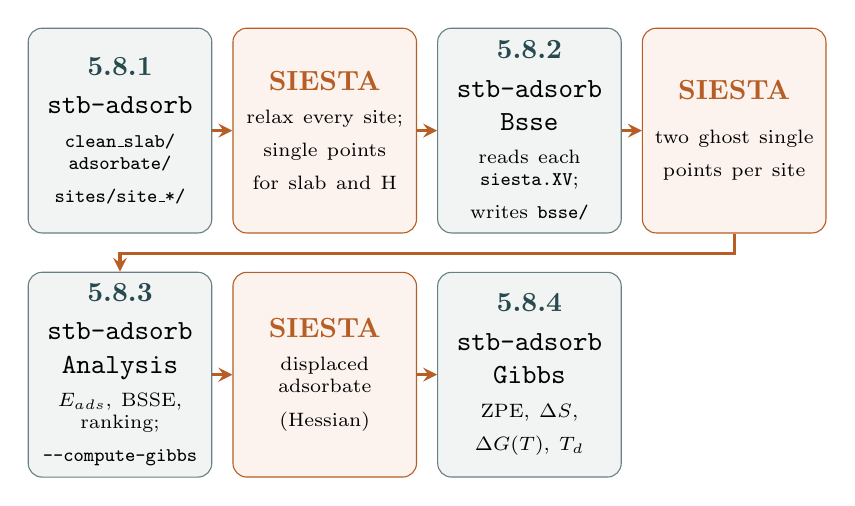
\begin{tikzpicture}[
		stage/.style={draw=stbteal!70,fill=stbteal!6,rounded corners=5pt,
			text width=2.05cm,minimum height=2.6cm,align=center,inner sep=4pt},
		run/.style={stage,draw=stborange!85!black,fill=stborange!8},
		flow/.style={->,>=stealth,line width=1.2pt,draw=stborange!85!black}
	]
		\node[stage] (p) at (0,0) {
			{\color{stbteal}\bfseries 5.8.1}\\[2pt]\texttt{stb-adsorb}\\[4pt]
			{\scriptsize \texttt{clean\_slab/}\\\texttt{adsorbate/}\\\texttt{sites/site\_*/}}
		};
		\node[run] (r1) at (2.6,0) {
			{\color{stborange!85!black}\bfseries SIESTA}\\[4pt]
			{\scriptsize relax every site;\\single points for slab and H}
		};
		\node[stage] (b) at (5.2,0) {
			{\color{stbteal}\bfseries 5.8.2}\\[2pt]\texttt{stb-adsorb}\\\texttt{Bsse}\\[4pt]
			{\scriptsize reads each\\\texttt{siesta.XV};\\writes \texttt{bsse/}}
		};
		\node[run] (r2) at (7.8,0) {
			{\color{stborange!85!black}\bfseries SIESTA}\\[4pt]
			{\scriptsize two ghost single points per site}
		};
		\node[stage] (a) at (0,-3.1) {
			{\color{stbteal}\bfseries 5.8.3}\\[2pt]\texttt{stb-adsorb}\\\texttt{Analysis}\\[4pt]
			{\scriptsize $E_{\text{ads}}$, BSSE,\\ranking;\\\texttt{--compute-gibbs}}
		};
		\node[run] (r3) at (2.6,-3.1) {
			{\color{stborange!85!black}\bfseries SIESTA}\\[4pt]
			{\scriptsize displaced\\adsorbate\\(Hessian)}
		};
		\node[stage] (g) at (5.2,-3.1) {
			{\color{stbteal}\bfseries 5.8.4}\\[2pt]\texttt{stb-adsorb}\\\texttt{Gibbs}\\[4pt]
			{\scriptsize ZPE, $\Delta S$,\\$\Delta G(T)$, $T_d$}
		};
		\draw[flow] (p) -- (r1); \draw[flow] (r1) -- (b);
		\draw[flow] (b) -- (r2); \draw[flow] (r2.south) -- ++(0,-0.25) -| (a.north);
		\draw[flow] (a) -- (r3); \draw[flow] (r3) -- (g);
	\end{tikzpicture}%
	}
	\vspace{0.3cm}
	\begin{columns}[T]
		\begin{column}{0.48\textwidth}
			\metroset{block=fill}
			\begin{block}{Starting point}
				\ttfamily\scriptsize
				stb-supercell -f structure.fdf -d 4 4 1 \textbackslash\\
				\ \ -o structure.fdf\\
				stb-inputfile structure.fdf -t relax -p dojo\\[2pt]
				\normalfont\scriptsize then set \texttt{kgrid.MonkhorstPack [3 3 1]}
			\end{block}
		\end{column}
		\begin{column}{0.48\textwidth}
			\metroset{block=fill}
			\begin{alertblock}{Why BSSE is a separate stage}
				\small
				\begin{itemize}
					\item Ghost runs need the \emph{relaxed} site geometry
					\item It exists only after the first SIESTA round
				\end{itemize}
			\end{alertblock}
		\end{column}
	\end{columns}
\end{frame}

%-------------------------------------------------
% SLIDE 2.5.7 - stb-adsorb
%-------------------------------------------------
\begin{frame}[fragile]{\texttt{stb-adsorb}: Sites and Reference Folders}
	\begin{columns}[T]
		\begin{column}{0.50\textwidth}
			{\scriptsize
\begin{verbatim}
stb-adsorb -s structure.fdf -c calc.fdf -p dojo \
  --adsorbate H --site-type all --all-sites \
  --height 1.5 -O adsorption_run --save-report
\end{verbatim}
			}
			\metroset{block=fill}
			\begin{block}{Site search (pymatgen)}
				\begin{tabular}{lrr}
					\toprule
					Type & Raw & Distinct \\
					\midrule
					ontop & 32 & 2 \\
					bridge & 96 & 4 \\
					hollow & 0 & 0 \\
					\midrule
					Total & 128 & \textbf{6} \\
					\bottomrule
				\end{tabular}
			\end{block}
			\begin{block}{Also written}
				\texttt{config\_extra.fdf} per folder (spin, D3, dipole, fixed cell),
				\texttt{site\_positions.dat}, \texttt{adsorption\_sites.png}
			\end{block}
		\end{column}
		\begin{column}{0.48\textwidth}
			\centering
			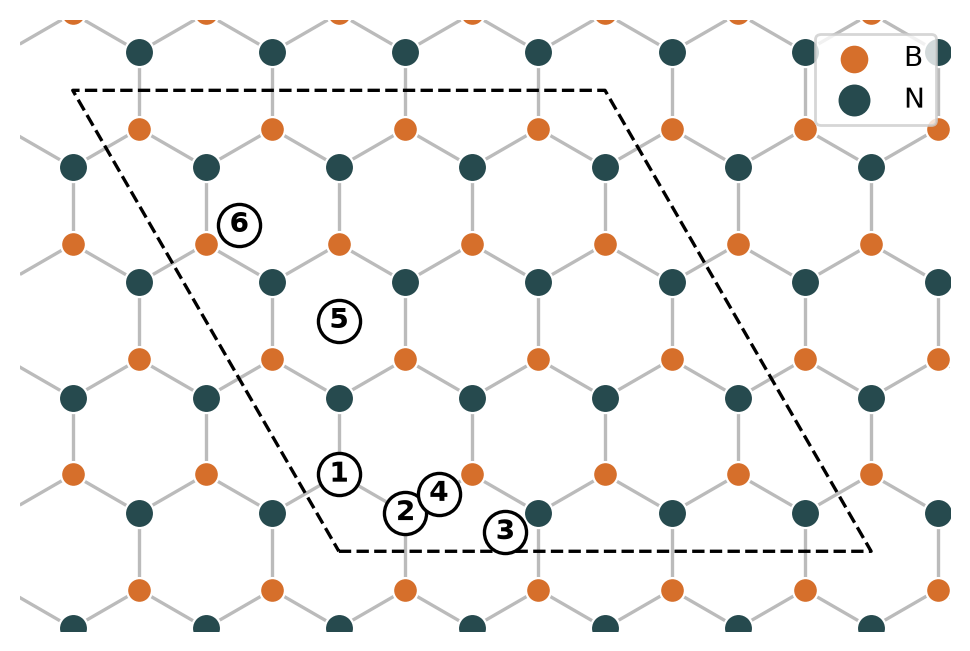
\includegraphics[width=\textwidth]{figures/hbn_adsorption_sites.png}
			\par\vspace{0.05cm}
			{\scriptsize 1: on B \quad 2: on N \quad 4: B--N bond \quad
			5: hexagon center\\3, 6: between an atom and the center}
			\par\vspace{0.1cm}
			\metroset{block=fill}
			\begin{alertblock}{Check the labels}
				\small
				\begin{itemize}
					\item On a honeycomb, the hollow appears as ``bridge'' 5
					\item Read the map, not only the names
				\end{itemize}
			\end{alertblock}
		\end{column}
	\end{columns}
\end{frame}

%-------------------------------------------------
% SLIDE 2.5.8 - stb-adsorbBsse
%-------------------------------------------------
\begin{frame}[fragile]{\texttt{stb-adsorbBsse}: Ghost Folders at the Relaxed Geometry}
	\begin{columns}[T]
		\begin{column}{0.50\textwidth}
			{\scriptsize
\begin{verbatim}
stb-adsorbBsse --dir adsorption_run --save-report
\end{verbatim}
			}
			\metroset{block=fill}
			\begin{block}{What it does}
				\begin{itemize}
					\item Reads each finished \texttt{sites/site\_*/siesta.XV}
					\item Flags sites whose residual force is above tolerance
					\item Writes \texttt{bsse/site\_*/bsse\_slab/} and \texttt{bsse\_adsorbate/}
					\item Inherits spin, D3, and dipole settings from the site
				\end{itemize}
			\end{block}
		\end{column}
		\begin{column}{0.46\textwidth}
			\metroset{block=fill}
			\begin{block}{h-BN report}
				\centering\small
				\begin{tabular}{lrl}
					\toprule
					Site & $F_{\max}$ (eV/\AA) & Status \\
					\midrule
					site\_1\_ontop  & 0.005 & ready \\
					site\_2\_ontop  & 0.008 & ready \\
					site\_3\_bridge & 0.010 & ready \\
					site\_4\_bridge & 0.009 & ready \\
					site\_5\_bridge & 0.007 & ready \\
					site\_6\_bridge & \textcolor{stborange}{0.016} & ready \\
					\bottomrule
				\end{tabular}
				\par\vspace{0.1cm}
				{\scriptsize 6 pairs $\rightarrow$ 12 single points (about 2~min each, 4 cores)}
			\end{block}
			{\scriptsize site\_6 stopped at the 150-step limit: still below the
			0.05~eV/\AA\ warning threshold.}
		\end{column}
	\end{columns}
\end{frame}

%-------------------------------------------------
% SLIDE 2.5.9 - stb-adsorbAnalysis
%-------------------------------------------------
\begin{frame}[fragile]{\texttt{stb-adsorbAnalysis}: Energies, BSSE, and Ranking}
	\begin{columns}[T]
		\begin{column}{0.38\textwidth}
			{\scriptsize
\begin{verbatim}
stb-adsorbAnalysis --dir adsorption_run \
  --save-report \
  --apply best_adsorbed_structure.fdf
\end{verbatim}
			}
			\metroset{block=fill}
			\begin{block}{What it reports}
				\begin{itemize}
					\item $E_{\text{ads}}$ per site, uncorrected and BSSE-corrected
					\item Residual-force check per site
					\item Ranking plot and \texttt{adsorption\_curve.dat}
					\item \texttt{--apply}: copies the best site's structure
				\end{itemize}
			\end{block}
		\end{column}
		\begin{column}{0.60\textwidth}
			\metroset{block=fill}
			\begin{block}{h-BN: $E_{\text{ads}}$ per site (eV, vs.\ atomic H)}
				\centering\scriptsize
				\setlength{\tabcolsep}{4pt}
				\begin{tabular}{llrrr}
					\toprule
					Site & Final state & raw & CP (STB) & CP + def. \\
					\midrule
					site\_1 & \textcolor{stborange}{B--H} & $-0.093$ & $\mathbf{-0.437}$ & $-0.007$ \\
					site\_4 & \textcolor{stborange}{B--H} & $-0.104$ & $-0.436$ & $\approx$ site\_1 \\
					site\_3 & phys. & $-0.107$ & $-0.034$ & $\mathbf{-0.049}$ \\
					site\_6 & phys. & $-0.103$ & $-0.033$ & \\
					site\_5 & phys. & $-0.093$ & $-0.033$ & \\
					site\_2 & phys. & $-0.079$ & $-0.029$ & \\
					\bottomrule
				\end{tabular}
			\end{block}
			\begin{alertblock}{Deformation energy}
				For B--H, the slab relaxes (B moves 0.32~\AA\ out of plane), which costs
				+0.43~eV. \textbf{CP (STB)} computes $E_{\text{site}}-E_{\text{slab}}^{[\text{ghost}]}-E_{\text{H}}^{[\text{ghost}]}$
				with the \emph{deformed} slab, so this cost is lost.
				Adding it back, physisorption wins.
			\end{alertblock}
		\end{column}
	\end{columns}
\end{frame}

%-------------------------------------------------
% SLIDE 2.5.9b - Stage 4: Gibbs
%-------------------------------------------------
\begin{frame}[fragile]{Stage 4: \texttt{stb-adsorbGibbs}}
	\begin{columns}[T]
		\begin{column}{0.50\textwidth}
			{\scriptsize
\begin{verbatim}
# Stage 3b: Hessian folders for the best site
stb-adsorbAnalysis --dir adsorption_run \
  --compute-gibbs --zpe-mode local
# run SIESTA in adsorption_run/gibbs/*/disp_*/
stb-adsorbGibbs --dir adsorption_run \
  --tmin 200 --tmax 800 --tstep 50 --save-report
\end{verbatim}
			}
			\metroset{block=fill}
			\begin{block}{Options}
				\begin{itemize}
					\item \texttt{local}: only the adsorbate moves; 6 displacements per atom
						(6 SIESTA runs for H)
					\item \texttt{full}: Phonopy on site and clean slab; $6\times3N$ runs
					\item \texttt{--displacement} (default 0.015~\AA)
				\end{itemize}
			\end{block}
			{\scriptsize Reports $D_0$, $\Delta$ZPE, $\Delta S$ (J/(mol\,K)), $\Delta G(T)$,
			$T_d$, and a rough desorption time.}
		\end{column}
		\begin{column}{0.46\textwidth}
			\centering
			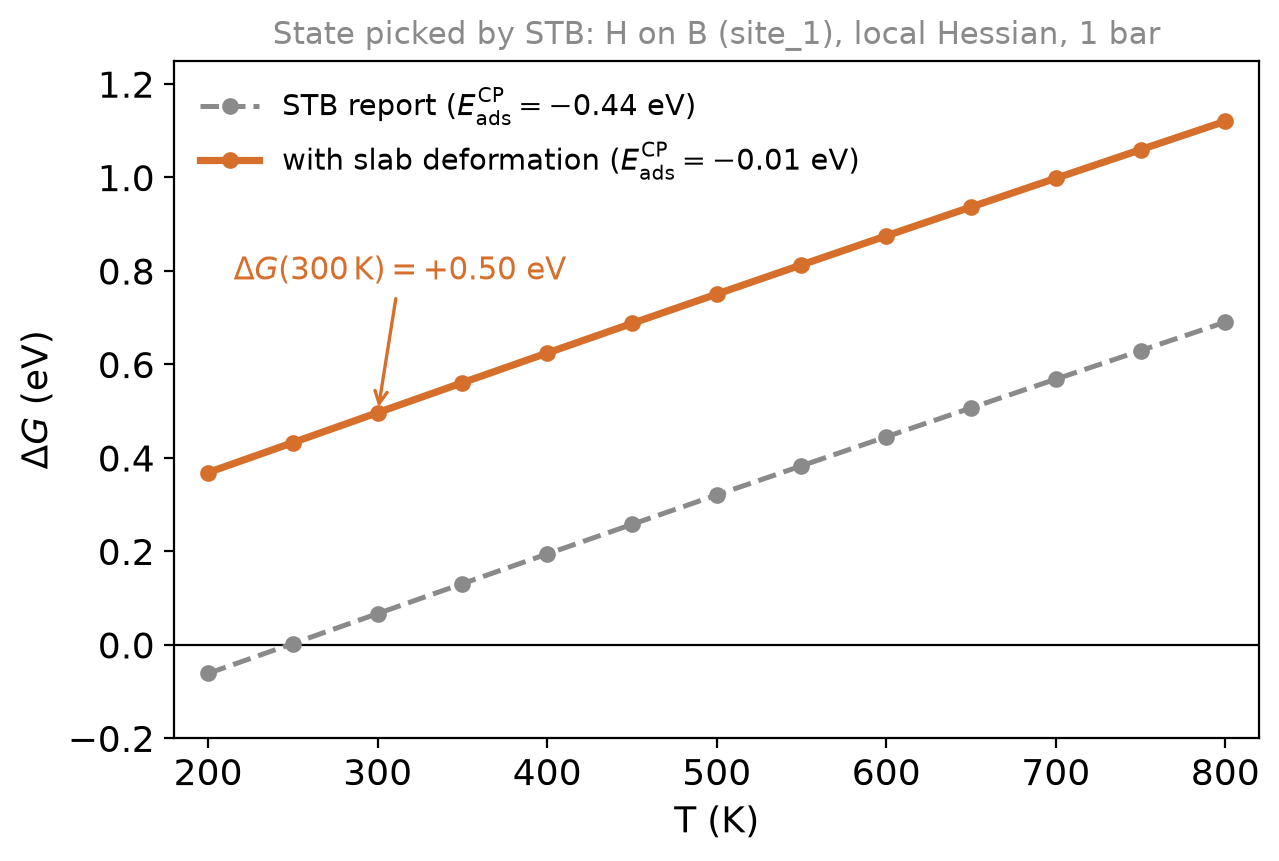
\includegraphics[width=\textwidth]{figures/hbn_ads_gibbs.png}
			\par\vspace{0.05cm}
			{\scriptsize
			\begin{tabular}{ll}
				H modes on B & 650, 650, 1224~cm$^{-1}$ (no imaginary) \\
				$\Delta$ZPE & $+0.16$~eV \\
				$\Delta S$ (300~K) & $-112$~J/(mol\,K) \\
				$-T\Delta S$ (300~K) & $+0.35$~eV \\
			\end{tabular}}
			\par\vspace{0.1cm}
			\metroset{block=fill}
			\begin{alertblock}{B--H is not stable on pristine h-BN}
				\small
				\begin{itemize}
					\item With slab deformation: $\Delta G > 0$ at all $T$
					\item Relative to $\tfrac{1}{2}$H$_2$: every site $\approx +2$~eV
				\end{itemize}
			\end{alertblock}
		\end{column}
	\end{columns}
\end{frame}

%-------------------------------------------------
% SLIDE 2.5.10 - Reading the result
%-------------------------------------------------
\begin{frame}{Reading the Result: Where Did H Go?}
	\centering
	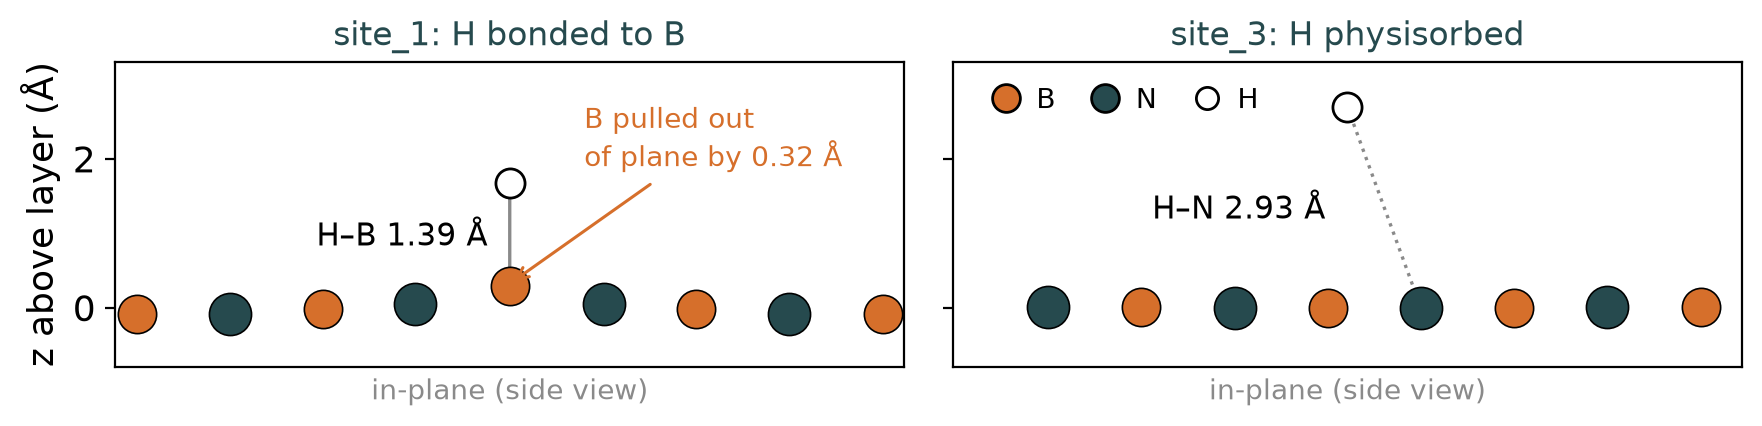
\includegraphics[width=0.92\textwidth]{figures/hbn_ads_geometry.png}
	\par\vspace{0.1cm}
	\begin{columns}[T]
		\begin{column}{0.48\textwidth}
			\metroset{block=fill}
			\begin{block}{Checklist on h-BN}
				\small
				\begin{itemize}
					\item \textbf{Final vs start:} site\_4 (B--N bridge) moved onto B,
						same state as site\_1; the others went to $\sim$2.7~\AA
					\item \textbf{Spin:} 1~$\mu_B$ in every site, so it does not separate the two states
					\item \textbf{BSSE:} $+0.06$ to $+0.09$~eV, as large as $E_{\text{ads}}$ itself
				\end{itemize}
			\end{block}
		\end{column}
		\begin{column}{0.48\textwidth}
			\metroset{block=fill}
			\begin{block}{Two basins, almost degenerate}
				\small
				Chemisorbed B--H and physisorbed H differ by only $\sim$0.04~eV.
				site\_1 and site\_4 (same structure) differ by 11~meV:
				that is the numerical noise level.
			\end{block}
		\end{column}
	\end{columns}
\end{frame}

%%%%%%%%%%%%%%%%%%%%%%%%%%%%%%%%%%%%%%%%%%%%%%%%%%%%%%%%
\section{Hands-on: H Adsorption on h-BN}
%%%%%%%%%%%%%%%%%%%%%%%%%%%%%%%%%%%%%%%%%%%%%%%%%%%%%%%%

%%%%%%%%%%%%%%%%%%%%%%%%%%%%%%%%%%%%%%%%%%%%%%%%%%%%%%%%
\section{Elastic Constants: Symmetry at Work}
%%%%%%%%%%%%%%%%%%%%%%%%%%%%%%%%%%%%%%%%%%%%%%%%%%%%%%%%

%-------------------------------------------------
% SLIDE 2.6.1 - Theory: Hooke's law in Voigt notation
%-------------------------------------------------
\begin{frame}{Hooke's Law in Voigt Notation}
	\begin{columns}[T]
		\begin{column}{0.50\textwidth}
			\[
				\sigma_i = \sum_{j=1}^{6} C_{ij}\,\gamma_j
			\]
			\[
				\gamma = (\varepsilon_{xx},\varepsilon_{yy},\varepsilon_{zz},
				2\varepsilon_{yz},2\varepsilon_{xz},2\varepsilon_{xy})
			\]
			\centering\small
			\begin{tabular}{cccccc}
				\toprule
				1 & 2 & 3 & 4 & 5 & 6 \\
				$xx$ & $yy$ & $zz$ & $yz$ & $xz$ & $xy$ \\
				\bottomrule
			\end{tabular}
			\par\vspace{0.2cm}\raggedright
			$C$ is a symmetric $6\times6$ matrix: at most \textbf{21} independent constants.
			\par\vspace{0.2cm}
			\metroset{block=fill}
			\begin{block}{Units depend on dimensionality}
				3D: GPa\quad 2D: N/m ($\sigma\cdot L_z$, independent of the vacuum)\quad 1D: nN
			\end{block}
		\end{column}
		\begin{column}{0.46\textwidth}
			\metroset{block=fill}
			\begin{block}{Stress method (default)}
				Strain one component, read SIESTA's stress tensor:
				one series gives a whole \textbf{column} of $C$.
				\[ C_{ij} = \partial\sigma_i/\partial\gamma_j \]
			\end{block}
			\begin{block}{Energy method}
				\[ E = E_0 + \tfrac{V_0}{2}\,\gamma^{T} C\,\gamma \]
				One curvature per pattern: off-diagonal terms need combined
				patterns such as $xx{+}yy$.
			\end{block}
		\end{column}
	\end{columns}
\end{frame}

%-------------------------------------------------
% SLIDE 2.6.2 - Theory: Neumann's principle
%-------------------------------------------------
\begin{frame}{Neumann's Principle: Symmetry Fixes the Pattern of $C$}
	\centering
	$C$ must be invariant under every operation $R$ of the point group:
	\[
		C'_{ijkl} = R_{ia}R_{jb}R_{kc}R_{ld}\,C_{abcd} = C_{ijkl}
	\]
	\begin{columns}[T]
		\begin{column}{0.53\textwidth}
			\metroset{block=fill}
			\begin{block}{GaAs, zincblende ($\bar{4}3m$): 3 constants}
				\centering\small
				$\begin{pmatrix}
					C_{11} & C_{12} & C_{12} & 0 & 0 & 0 \\
					C_{12} & C_{11} & C_{12} & 0 & 0 & 0 \\
					C_{12} & C_{12} & C_{11} & 0 & 0 & 0 \\
					0 & 0 & 0 & C_{44} & 0 & 0 \\
					0 & 0 & 0 & 0 & C_{44} & 0 \\
					0 & 0 & 0 & 0 & 0 & C_{44}
				\end{pmatrix}$
			\end{block}
		\end{column}
		\begin{column}{0.43\textwidth}
			\metroset{block=fill}
			\begin{block}{h-BN monolayer ($\bar{6}m2$), in plane}
				\centering\small
				$\begin{pmatrix}
					C_{11} & C_{12} & 0 \\
					C_{12} & C_{11} & 0 \\
					0 & 0 & \tfrac{C_{11}-C_{12}}{2}
				\end{pmatrix}$
				\par\vspace{0.15cm}
				{\scriptsize 2 in-plane constants (5 for the full 3D tensor)}
			\end{block}
		\end{column}
	\end{columns}
	\vspace{0.2cm}
	\metroset{block=fill}
	\begin{alertblock}{Fewer constants, fewer calculations}
		\small
		\begin{itemize}
			\item Triclinic: 21 constants, 6 strain series
			\item Cubic: 3 constants, 2 series \quad Hexagonal 2D: 1 series
		\end{itemize}
	\end{alertblock}
\end{frame}

%-------------------------------------------------
% SLIDE 2.6.3 - Theory: how STB implements symmetry
%-------------------------------------------------
\begin{frame}{How STB Uses the Point Group}
	\relax
	{\small Point group from pymatgen (\texttt{SpacegroupAnalyzer}), operations
	$R$ in \textbf{Cartesian} coordinates.}
	\par\vspace{0.15cm}
	\begin{columns}[T]
		\begin{column}{0.48\textwidth}
			\metroset{block=fill}
			\begin{block}{\texttt{--symmetry-method basic}}
				Pairwise test on the strain tensors:
				\[ R\,\varepsilon^{(i)}R^{T} = \pm\,\varepsilon^{(j)} \]
				If true, direction $j$ is skipped and its stress is rebuilt:
				\[ \sigma^{(j)} = \pm\,R\,\sigma^{(i)}R^{T} \]
				{\scriptsize Cubic: $\{xx,yy,zz\}$, $\{yz,xz,xy\}$.
				Hexagonal: a $60^\circ$ rotation sends $\varepsilon_{xx}$ to a
				\emph{mixed} tensor, so $C_{11}=C_{22}$ is \textbf{missed}.}
			\end{block}
		\end{column}
		\begin{column}{0.48\textwidth}
			\metroset{block=fill}
			\begin{block}{\texttt{--symmetry-method full}}
				Write $C$ as 21 unknowns $c$; each $R$ gives a linear map $L_R$:
				\[ (L_R - I)\,c = 0 \quad \forall R \]
				SVD null space $\rightarrow$ basis $\{B_k\}$, one per independent constant.
				\[ \sigma = \textstyle\sum_k x_k\,B_k\,\gamma \]
				{\scriptsize Directions chosen greedily until the design matrix reaches
				rank $K$; one global least-squares fit for all $x_k$.}
			\end{block}
		\end{column}
	\end{columns}
	\vspace{0.15cm}
	{\scriptsize Source: \texttt{stb/core/symmetry.py}
	(\texttt{equivalent\_strain\_modes}, \texttt{symmetry\_allowed\_basis},
	\texttt{select\_directions\_by\_rank}, \texttt{fit\_stiffness\_matrix}).}
\end{frame}

%-------------------------------------------------
% SLIDE 2.6.4 - Theory: frame matters
%-------------------------------------------------
\begin{frame}{Symmetry Lives in the Cartesian Frame}
	\begin{columns}[T]
		\begin{column}{0.50\textwidth}
			Voigt strains are applied along Cartesian $x,y,z$.
			The reduction works only if these axes match the crystal axes.
			\par\vspace{0.2cm}
			\metroset{block=fill}
			\begin{block}{Same GaAs, two cells (Stage 1 only)}
				\centering\small
				\begin{tabular}{lcc}
					\toprule
					Cell & \texttt{basic} & \texttt{full} \\
					\midrule
					cubic axes & 2 of 6 & 2 of 6 \\
					Part 1 cell (rotated) & 6 of 6 & 1 of 6 \\
					\bottomrule
				\end{tabular}
			\end{block}
			{\small Both detect $\bar{4}3m$, but in the rotated frame $C$ has extra
			nonzero entries: $C_{11}$ there is \emph{not} the textbook $C_{11}$.}
		\end{column}
		\begin{column}{0.46\textwidth}
			\metroset{block=fill}
			\begin{block}{Standard zincblende cell}
				\small
				\[
					\mathbf{a}_1 = \tfrac{a}{2}(0,1,1),\
					\mathbf{a}_2 = \tfrac{a}{2}(1,0,1),\
					\mathbf{a}_3 = \tfrac{a}{2}(1,1,0)
				\]
				Ga $(0,0,0)$, As $(\tfrac14,\tfrac14,\tfrac14)$
			\end{block}
			\begin{alertblock}{Before Stage 1}
				Check that the reported point group is the expected one
				($\bar{4}3m$, $\bar{6}m2$) and that the cell is in the standard orientation.
				Do not raise \texttt{--symprec} to hide a distorted cell.
			\end{alertblock}
		\end{column}
	\end{columns}
\end{frame}

%-------------------------------------------------
% SLIDE 2.6.5 - Theory: internal strain
%-------------------------------------------------
\begin{frame}{Clamped Ion vs Relaxed Ion: Symmetry Decides}
	\begin{columns}[T]
		\begin{column}{0.50\textwidth}
			\metroset{block=fill}
			\begin{block}{Internal strain}
				With 2+ atoms per cell, a strain can push the sublattices against each other.
				STB forces \texttt{MD.Steps 0}: ions stay at the scaled positions
				$\Rightarrow$ \textbf{clamped-ion} $C_{ij}$.
			\end{block}
			\begin{block}{When does it happen?}
				\small
				\begin{tabular}{lll}
					\toprule
					Strain & GaAs & h-BN \\
					\midrule
					$xx$ & $F = 0.0001$ & $F = 0.13$ \\
					$xy$ & $F = 0.13$ & $F = 0.28$ \\
					\bottomrule
				\end{tabular}
				\par{\scriptsize Max force (eV/\AA) at 1\% strain.
				Only strain with the symmetry of the sublattice mode couples:
				$T_2$ (shear) in $T_d$; $E'$ ($\varepsilon_{xx}-\varepsilon_{yy}$,
				$\varepsilon_{xy}$) in $D_{3h}$. h-BN biaxial strain ($A_1'$):
				$F = 5\times10^{-5}$.}
			\end{block}
		\end{column}
		\begin{column}{0.46\textwidth}
			\metroset{block=fill}
			\begin{block}{Relaxing the ions (cell fixed)}
				\centering\small
				\begin{tabular}{lrr}
					\toprule
					& clamped & relaxed \\
					\midrule
					GaAs $C_{11}$ (GPa) & 94.1 & 94.1 \\
					GaAs $C_{44}$ (GPa) & 64.2 & \textbf{47.5} \\
					\midrule
					h-BN $C_{11}$ (N/m) & 307.3 & \textbf{294.2} \\
					h-BN $C_{12}$ (N/m) & 54.2 & \textbf{67.4} \\
					h-BN $C_{11}+C_{12}$ & 361.5 & 361.6 \\
					\bottomrule
				\end{tabular}
			\end{block}
			\begin{alertblock}{Compare with experiment: relaxed ion}
				STB has no relaxed-ion option: here \texttt{config\_extra.fdf} was
				edited by hand (\texttt{MD.Steps 100}).
			\end{alertblock}
		\end{column}
	\end{columns}
\end{frame}

%-------------------------------------------------
% SLIDE 2.6.6 - Theory: precision for stress
%-------------------------------------------------
\begin{frame}{Elastic Constants Need More Convergence}
	\begin{columns}[T]
		\begin{column}{0.46\textwidth}
			\centering
			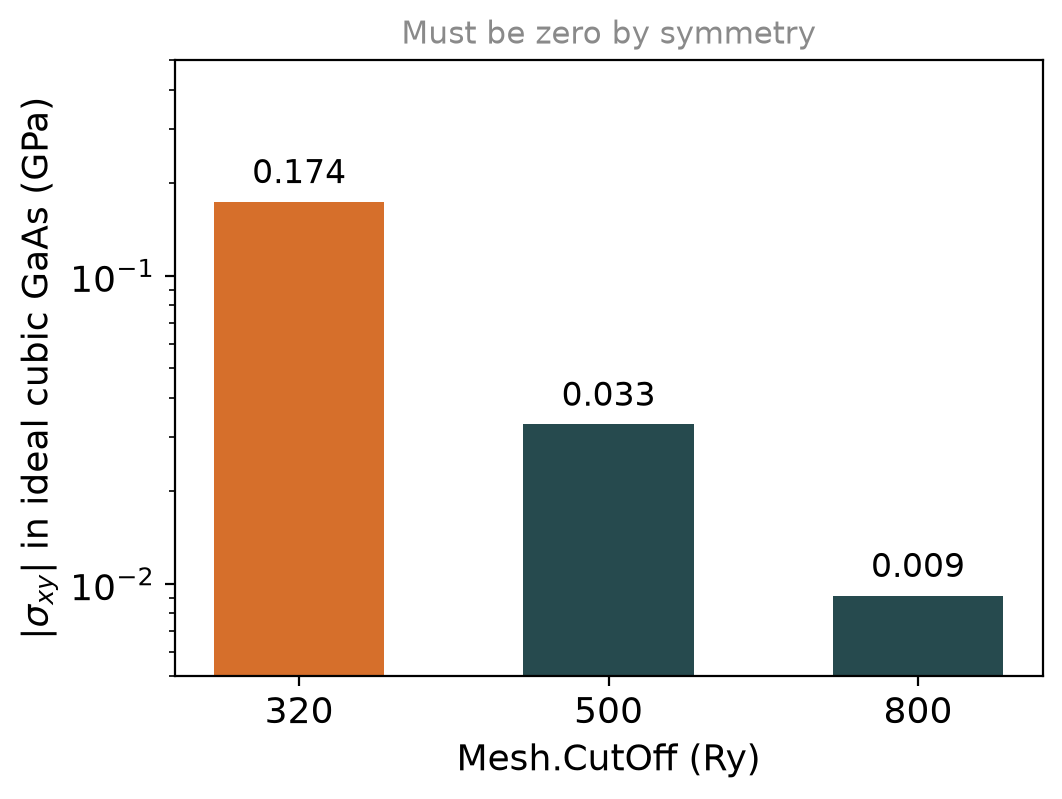
\includegraphics[width=0.9\textwidth]{figures/elastic_eggbox_mesh.png}
			\par\vspace{0.05cm}
			{\scriptsize Egg-box: the real-space grid of the FCC cell has only
			trigonal symmetry, so it creates a shear stress that $\bar{4}3m$ forbids.}
		\end{column}
		\begin{column}{0.52\textwidth}
			\centering
			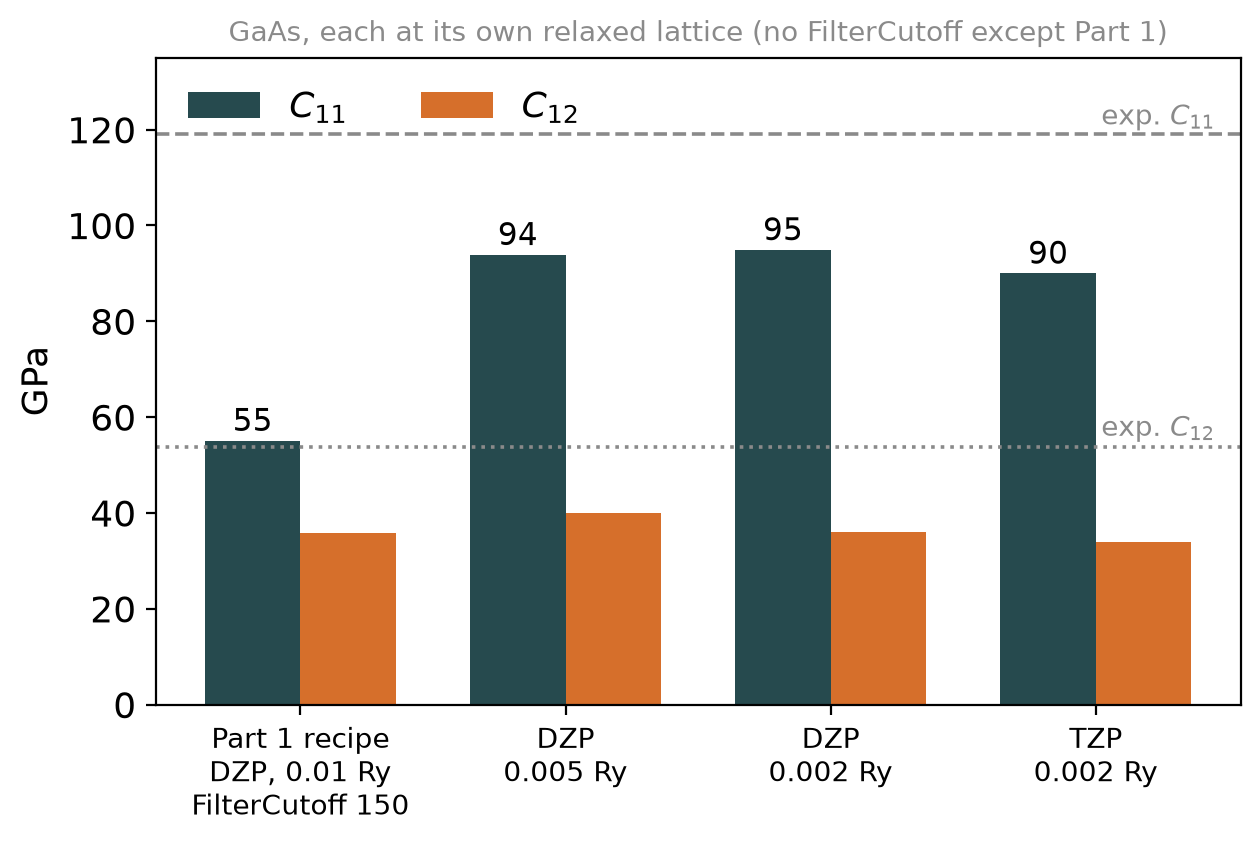
\includegraphics[width=\textwidth]{figures/elastic_basis_conv.png}
		\end{column}
	\end{columns}
	\vspace{0.1cm}
	\begin{columns}[T]
		\begin{column}{0.48\textwidth}
			\metroset{block=fill}
			\begin{block}{Reference structure}
				\texttt{MD.MaxStressTol 0.01 GPa} (default: 1~GPa).
				The Part 1 GaAs cell kept $\sim$1~GPa of residual stress.
			\end{block}
		\end{column}
		\begin{column}{0.48\textwidth}
			\metroset{block=fill}
			\begin{alertblock}{Part 1 recipe: $C_{11}$ 40\% too low}
				\small
				\begin{itemize}
					\item \texttt{FilterCutoff} + \texttt{EnergyShift 0.01 Ry} soften Ga 3d
					\item Used here: DZP, 0.005~Ry, no filter, 500~Ry
				\end{itemize}
			\end{alertblock}
		\end{column}
	\end{columns}
\end{frame}

%-------------------------------------------------
% SLIDE 2.6.7 - Theory: stability and derived moduli
%-------------------------------------------------
\begin{frame}{Mechanical Stability and Derived Moduli}
	\begin{columns}[T]
		\begin{column}{0.48\textwidth}
			\metroset{block=fill}
			\begin{block}{Born stability: $C$ positive definite}
				\small
				Cubic:\quad $C_{11}-C_{12}>0,\ C_{11}+2C_{12}>0,\ C_{44}>0$
				\par\vspace{0.1cm}
				2D:\quad $C_{11}>0,\ C_{66}>0,\ C_{11}C_{22}>C_{12}^2$
				\par\vspace{0.1cm}
				{\scriptsize STB (3D): all eigenvalues of $C$ positive; works for any
				point group.}
			\end{block}
			\begin{block}{2D moduli}
				\small
				\[ Y_{2D} = \frac{C_{11}C_{22}-C_{12}^2}{C_{22}},\qquad
				\nu = \frac{C_{12}}{C_{22}} \]
			\end{block}
		\end{column}
		\begin{column}{0.48\textwidth}
			\metroset{block=fill}
			\begin{block}{3D moduli: Voigt--Reuss--Hill}
				\small
				\[ B_V = \tfrac{1}{9}\textstyle\sum_{i,j\le3}C_{ij} \qquad
				B_R = \Big(\textstyle\sum_{i,j\le3}S_{ij}\Big)^{-1} \]
				$B_H=\tfrac12(B_V+B_R)$, same for $G$; then
				\[ E = \frac{9BG}{3B+G},\qquad \nu = \frac{3B-2G}{2(3B+G)} \]
				{\scriptsize $S = C^{-1}$. Cubic: $B = (C_{11}+2C_{12})/3$.}
			\end{block}
			\begin{block}{Anisotropy}
				\small $A^U = 5G_V/G_R + B_V/B_R - 6$\quad (0 = isotropic)
			\end{block}
		\end{column}
	\end{columns}
\end{frame}

%-------------------------------------------------
% SLIDE 2.6.8 - Workflow 5.2
%-------------------------------------------------
\begin{frame}{Workflow 5.2: Elastic Constants with STB}
	\centering
	\resizebox{0.95\textwidth}{!}{%
	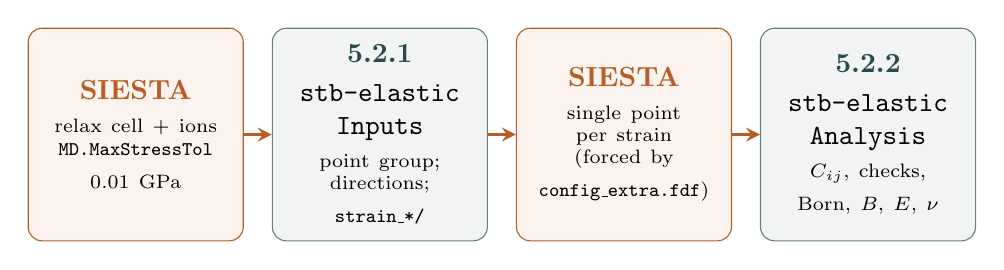
\begin{tikzpicture}[
		stage/.style={draw=stbteal!70,fill=stbteal!6,rounded corners=5pt,
			text width=2.45cm,minimum height=2.7cm,align=center,inner sep=4pt},
		run/.style={stage,draw=stborange!85!black,fill=stborange!8},
		flow/.style={->,>=stealth,line width=1.2pt,draw=stborange!85!black}
	]
		\node[run] (r0) at (0,0) {
			{\color{stborange!85!black}\bfseries SIESTA}\\[4pt]
			{\scriptsize relax cell + ions\\\texttt{MD.MaxStressTol}\\0.01 GPa}
		};
		\node[stage] (i) at (3.1,0) {
			{\color{stbteal}\bfseries 5.2.1}\\[2pt]\texttt{stb-elastic}\\\texttt{Inputs}\\[4pt]
			{\scriptsize point group;\\directions;\\\texttt{strain\_*/}}
		};
		\node[run] (r1) at (6.2,0) {
			{\color{stborange!85!black}\bfseries SIESTA}\\[4pt]
			{\scriptsize single point per strain\\(forced by\\\texttt{config\_extra.fdf})}
		};
		\node[stage] (a) at (9.3,0) {
			{\color{stbteal}\bfseries 5.2.2}\\[2pt]\texttt{stb-elastic}\\\texttt{Analysis}\\[4pt]
			{\scriptsize $C_{ij}$, checks,\\Born, $B$, $E$, $\nu$}
		};
		\draw[flow] (r0) -- (i); \draw[flow] (i) -- (r1); \draw[flow] (r1) -- (a);
	\end{tikzpicture}%
	}
	\vspace{0.3cm}
	\begin{columns}[T]
		\begin{column}{0.48\textwidth}
			\metroset{block=fill}
			\begin{block}{Choices made in Stage 1}
				\small
				\texttt{--method stress|energy}\\
				\texttt{--symmetry-method basic|full}\\
				\texttt{--max 1.0 --steps 5}\ (\(\pm1\%\), 5 points)
			\end{block}
		\end{column}
		\begin{column}{0.48\textwidth}
			\metroset{block=fill}
			\begin{alertblock}{Must match}
				\small
				\begin{itemize}
					\item Stage 2: same \texttt{--method} and \texttt{--symmetry-method}
					\item Point group from \texttt{reference\_structure.fdf} (undeformed cell)
				\end{itemize}
			\end{alertblock}
		\end{column}
	\end{columns}
\end{frame}

%-------------------------------------------------
% SLIDE 2.6.9 - stb-elasticInputs
%-------------------------------------------------
\begin{frame}[fragile]{\texttt{stb-elasticInputs}: Symmetry Picks the Directions}
	\relax
	{\scriptsize
\begin{verbatim}
stb-elasticInputs -s structure.fdf -c calc.fdf --dirs all \
  --symmetry-method full --max 1.0 --steps 5 -o elastic_stress_full --save-report
\end{verbatim}
	}
	\begin{columns}[T]
		\begin{column}{0.48\textwidth}
			\metroset{block=fill}
			\begin{block}{GaAs: point group $\bar{4}3m$, 24 operations}
				\centering\scriptsize
				\begin{tabular}{lll}
					\toprule
					Dir. & \texttt{basic} & \texttt{full} \\
					\midrule
					$xx$ & RUN & RUN \\
					$yy$, $zz$ & from $xx$ & fit \\
					$xy$ & RUN & RUN \\
					$xz$, $yz$ & from $xy$ & fit \\
					\midrule
					runs & 10 & 10 \\
					\bottomrule
				\end{tabular}
				\par\vspace{0.1cm}
				\texttt{energy}: $xx$, $yz$, $xx{+}yy$ (15 runs)
			\end{block}
		\end{column}
		\begin{column}{0.48\textwidth}
			\metroset{block=fill}
			\begin{block}{h-BN: point group $\bar{6}m2$, 12 operations}
				\centering\scriptsize
				\begin{tabular}{lll}
					\toprule
					Dir. & \texttt{basic} & \texttt{full} \\
					\midrule
					$xx$ & RUN & RUN \\
					$yy$ & RUN & fit \\
					$xy$ & RUN & fit \\
					$zz$, $xz$, $yz$ & \multicolumn{2}{l}{skipped: vacuum} \\
					\midrule
					runs & 15 & \textbf{5} \\
					\bottomrule
				\end{tabular}
				\par\vspace{0.1cm}
				\texttt{energy}: $xx$, $xy$ (10 runs)
			\end{block}
		\end{column}
	\end{columns}
	\vspace{0.1cm}
	{\scriptsize Every folder gets \texttt{config\_extra.fdf} (\texttt{MD.Steps 0},
	\texttt{MD.VariableCell false}) \texttt{\%include}d at the \emph{top} of \texttt{calc.fdf}:
	first occurrence wins.}
\end{frame}

%-------------------------------------------------
% SLIDE 2.6.10 - stb-elasticAnalysis: GaAs
%-------------------------------------------------
\begin{frame}[fragile]{\texttt{stb-elasticAnalysis}: GaAs}
	\relax
	{\scriptsize
\begin{verbatim}
stb-elasticAnalysis -d elastic_stress_full --symmetry-method full --save-report --save-gnuplot
\end{verbatim}
	}
	\begin{columns}[T]
		\begin{column}{0.56\textwidth}
			\metroset{block=fill}
			\begin{block}{Four routes, one tensor (GPa)}
				\centering\scriptsize
				\setlength{\tabcolsep}{4pt}
				\begin{tabular}{lrrrr}
					\toprule
					Run & runs & $C_{11}$ & $C_{12}$ & $C_{44}$ \\
					\midrule
					stress, \texttt{basic} & 10 & 94.1 & 40.0 & 64.2 \\
					stress, \texttt{full} & 10 & 94.1 & 40.0 & 64.2 \\
					stress, 6 explicit & 30 & 94.1 & 40.0 & 64.2 \\
					energy & 15 & 94.6 & 39.4 & 64.7 \\
					\midrule
					relaxed ion & 10 & 94.1 & 40.0 & \textbf{47.5} \\
					Exp.\ (RT) & & 118.8 & 53.8 & 59.4 \\
					\bottomrule
				\end{tabular}
			\end{block}
			{\scriptsize Relaxed ion: $B = 58$~GPa, $E = 93$~GPa, $\nu = 0.23$,
			Zener $2C_{44}/(C_{11}-C_{12}) = 1.76$ (exp.\ 1.83). STABLE.\\
			Exp.: Bateman, McSkimin \& Whelan, J.\ Appl.\ Phys.\ 30, 544 (1959).}
		\end{column}
		\begin{column}{0.40\textwidth}
			\metroset{block=fill}
			\begin{block}{[3] Quality checks}
				\scriptsize
				Egg-box (stress vs energy):\\ $xx$ 0.55\%, $xy$ 0.71\% \hfill OK\\[2pt]
				Fit: $R^2 \ge 0.996$ \hfill OK\\[2pt]
				$\max|C_{ij}-C_{ji}|$ (6 explicit): 0.04~GPa \hfill OK
			\end{block}
			\begin{alertblock}{Checks catch noise, not a bad model}
				The Part 1 recipe ($C_{11}=55$~GPa) also passes every check.
			\end{alertblock}
		\end{column}
	\end{columns}
\end{frame}

%-------------------------------------------------
% SLIDE 2.6.11 - stb-elasticAnalysis: h-BN
%-------------------------------------------------
\begin{frame}{\texttt{stb-elasticAnalysis}: h-BN}
	\begin{columns}[T]
		\begin{column}{0.56\textwidth}
			\metroset{block=fill}
			\begin{block}{In-plane constants (N/m)}
				\centering\scriptsize
				\setlength{\tabcolsep}{4pt}
				\begin{tabular}{lrrrrr}
					\toprule
					Run & runs & $C_{11}$ & $C_{22}$ & $C_{12}$ & $C_{66}$ \\
					\midrule
					stress, \texttt{basic} & 15 & 307.3 & 307.0 & 54.2 & 126.5 \\
					stress, \texttt{full} & 5 & 307.3 & 307.3 & 54.1 & 126.6 \\
					energy & 10 & 307.9 & 307.9 & 54.5 & 126.7 \\
					\midrule
					relaxed ion & 15 & 294.2 & 293.8 & 67.4 & 113.2 \\
					\bottomrule
				\end{tabular}
			\end{block}
			{\scriptsize Relaxed ion: $Y_{2D} = 279$~N/m, $\nu = 0.23$.
			The sublattice shift (also the origin of piezoelectricity in h-BN)
			lowers $C_{11}-C_{12}$ only [Michel \& Verberck, PRB 80, 224301 (2009)].}
		\end{column}
		\begin{column}{0.40\textwidth}
			\metroset{block=fill}
			\begin{block}{What \texttt{basic} buys}
				\small
				$C_{66}$ measured: 126.5\\
				$(C_{11}-C_{12})/2$: 126.5\\
				$C_{12}$ from $xx$ vs $yy$: $\Delta = 0.27$
				\par\vspace{0.1cm}
				{\scriptsize In \texttt{full}, all three are true by construction,
				so they test nothing.}
			\end{block}
			\begin{alertblock}{Cost}
				\texttt{full}: 3$\times$ cheaper, same numbers.
			\end{alertblock}
		\end{column}
	\end{columns}
\end{frame}

%-------------------------------------------------
% SLIDE 2.6.12 - Reading the fits
%-------------------------------------------------
\begin{frame}{Reading the Fits}
	\centering
	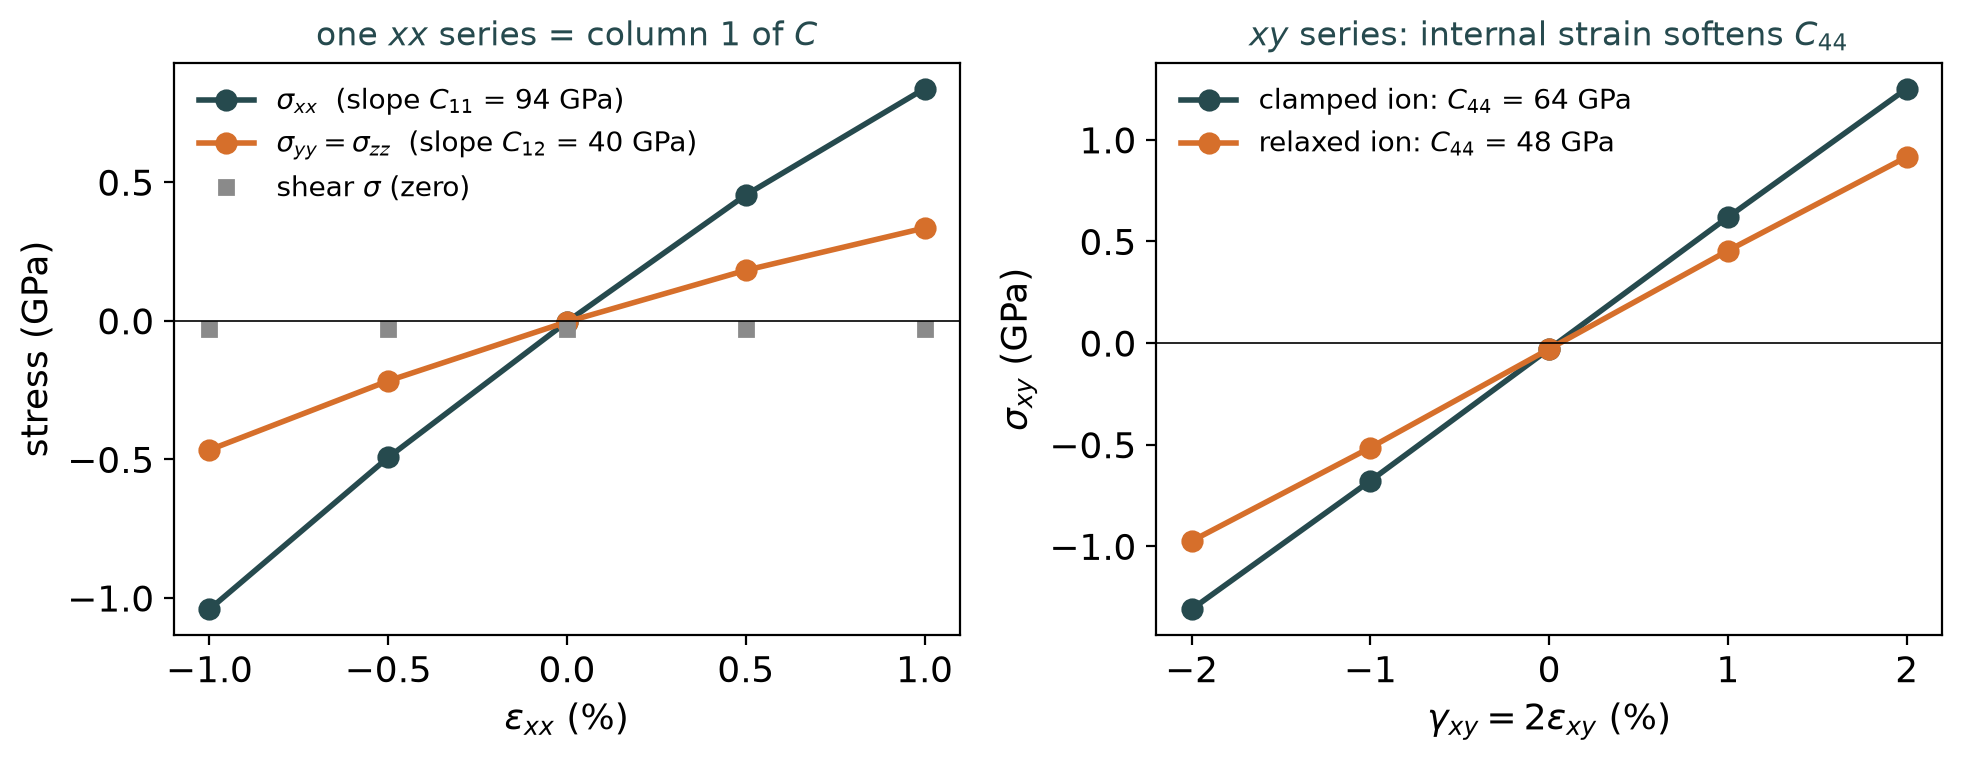
\includegraphics[width=0.95\textwidth]{figures/elastic_gaas_fits.png}
	\par\vspace{0.1cm}
	\begin{columns}[T]
		\begin{column}{0.48\textwidth}
			\metroset{block=fill}
			\begin{block}{Checklist}
				\small
				\begin{itemize}
					\item Linear within $\pm1\%$ ($R^2$)
					\item Zero-strain stress $\approx 0$ (relaxed reference)
					\item Forbidden components stay $\approx 0$
				\end{itemize}
			\end{block}
		\end{column}
		\begin{column}{0.48\textwidth}
			\metroset{block=fill}
			\begin{block}{Files}
				\small
				\texttt{elastic\_stage2.txt}, \texttt{elastic\_plots/*\_fit.dat}
				(columns: strain, $\gamma$, six $\sigma$ components)
			\end{block}
		\end{column}
	\end{columns}
\end{frame}

%%%%%%%%%%%%%%%%%%%%%%%%%%%%%%%%%%%%%%%%%%%%%%%%%%%%%%%%
\section{Hands-on: Elastic Constants of GaAs and h-BN}
%%%%%%%%%%%%%%%%%%%%%%%%%%%%%%%%%%%%%%%%%%%%%%%%%%%%%%%%

%%%%%%%%%%%%%%%%%%%%%%%%%%%%%%%%%%%%%%%%%%%%%%%%%%%%%%%%
\section{Closing}
%%%%%%%%%%%%%%%%%%%%%%%%%%%%%%%%%%%%%%%%%%%%%%%%%%%%%%%%

%-------------------------------------------------
% SLIDE 2.7.1 - Part 2 in six figures
%-------------------------------------------------
\begin{frame}{Part 2 in Six Figures}
	\centering
	\recapfig{gaas_bands.png}{Bands: FCC path, PBE gap}\hfill
	\recapfig{hbn_bands_pdos.png}{Bands + PDOS of h-BN}\hfill
	\recapfig{hbn_workfunction.png}{Work function, $E_F$ mid-gap}
	\par\vspace{0.25cm}
	\recapfig{gaas_fatbands.png}{Fatbands: orbital character}\hfill
	\recapfig{hbn_ads_gibbs.png}{H on h-BN: $\Delta G > 0$}\hfill
	\recapfig{elastic_gaas_fits.png}{$C_{ij}$: symmetry + internal strain}
	\par\vspace{0.3cm}
	{\small Every figure came from a SIESTA output read by one STB command.}
\end{frame}

%-------------------------------------------------
% SLIDE 2.7.2 - The course in one map
%-------------------------------------------------
\begin{frame}{The Course in One Map}
	\centering
	\resizebox{0.97\textwidth}{!}{%
	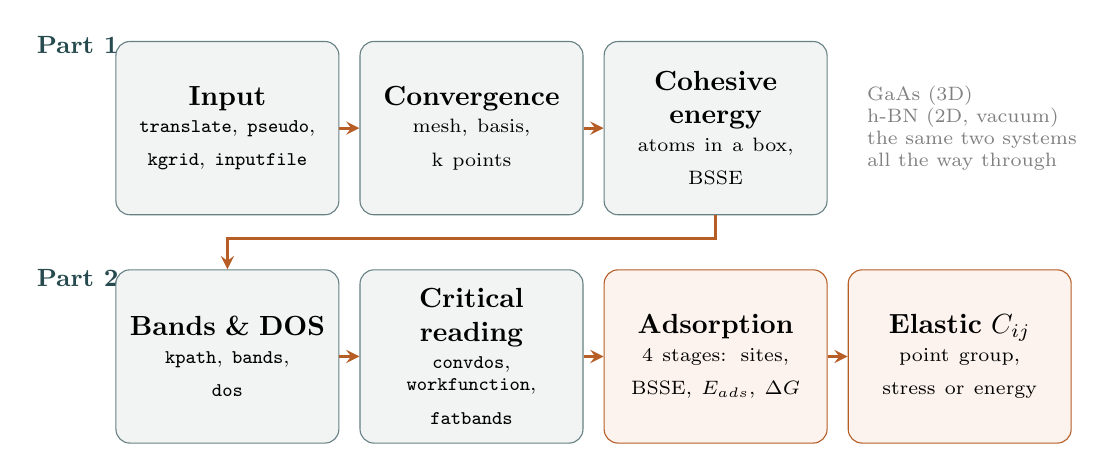
\begin{tikzpicture}[
		box/.style={draw=stbteal!70,fill=stbteal!6,rounded corners=5pt,
			text width=2.55cm,minimum height=2.2cm,align=center,inner sep=4pt},
		hot/.style={box,draw=stborange!85!black,fill=stborange!8},
		flow/.style={->,>=stealth,line width=1.1pt,draw=stborange!85!black},
		lab/.style={font=\bfseries\small,text=stbteal}
	]
		\node[lab] at (-1.9,1.05) {Part 1};
		\node[box] (a) at (0,0) {{\bfseries Input}\\[2pt]{\scriptsize\texttt{translate}, \texttt{pseudo},\\\texttt{kgrid}, \texttt{inputfile}}};
		\node[box] (b) at (3.1,0) {{\bfseries Convergence}\\[2pt]{\scriptsize mesh, basis,\\k points}};
		\node[box] (c) at (6.2,0) {{\bfseries Cohesive energy}\\[2pt]{\scriptsize atoms in a box,\\BSSE}};
		\node[lab] at (-1.9,-1.9) {Part 2};
		\node[box] (d) at (0,-2.9) {{\bfseries Bands \& DOS}\\[2pt]{\scriptsize \texttt{kpath}, \texttt{bands},\\\texttt{dos}}};
		\node[box] (e) at (3.1,-2.9) {{\bfseries Critical reading}\\[2pt]{\scriptsize \texttt{convdos}, \texttt{workfunction},\\\texttt{fatbands}}};
		\node[hot] (f) at (6.2,-2.9) {{\bfseries Adsorption}\\[2pt]{\scriptsize 4 stages: sites,\\BSSE, $E_{\text{ads}}$, $\Delta G$}};
		\node[hot] (g) at (9.3,-2.9) {{\bfseries Elastic $C_{ij}$}\\[2pt]{\scriptsize point group,\\stress or energy}};
		\draw[flow] (a) -- (b); \draw[flow] (b) -- (c);
		\draw[flow] (c.south) -- ++(0,-0.3) -| (d.north);
		\draw[flow] (d) -- (e); \draw[flow] (e) -- (f); \draw[flow] (f) -- (g);
		\node[font=\scriptsize,text=gray,align=left,anchor=west] at (8.0,0) {GaAs (3D)\\h-BN (2D, vacuum)\\the same two systems\\all the way through};
	\end{tikzpicture}%
	}
	\vspace{0.25cm}
	\begin{columns}[T]
		\begin{column}{0.48\textwidth}
			\metroset{block=fill}
			\begin{block}{Single tools}
				One output $\rightarrow$ one property
				(bands, DOS, work function, fatbands).
			\end{block}
		\end{column}
		\begin{column}{0.48\textwidth}
			\metroset{block=fill}
			\begin{block}{Workflows (orange)}
				Several SIESTA rounds; each stage reads the previous one
				and writes the next folders.
			\end{block}
		\end{column}
	\end{columns}
\end{frame}

%-------------------------------------------------
% SLIDE 2.7.3 - One pattern
%-------------------------------------------------
\begin{frame}{One Pattern for Every Property}
	\begin{columns}[c]
		\begin{column}{0.50\textwidth}
			\centering
			\resizebox{\textwidth}{!}{%
			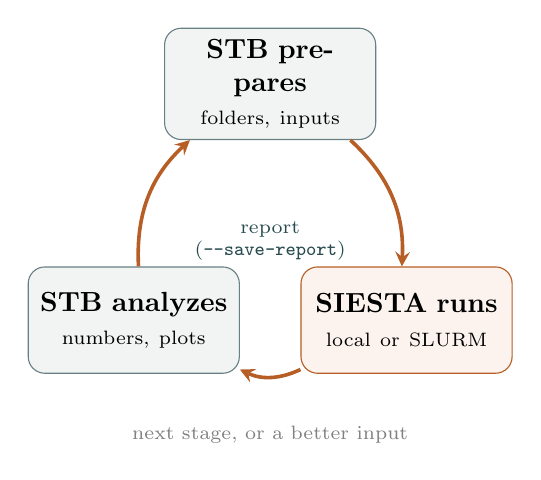
\begin{tikzpicture}[
				node/.style={draw=stbteal!70,fill=stbteal!6,rounded corners=6pt,
					text width=2.4cm,minimum height=1.35cm,align=center,inner sep=4pt},
				run/.style={node,draw=stborange!85!black,fill=stborange!8},
				flow/.style={->,>=stealth,line width=1.3pt,draw=stborange!85!black}
			]
				\node[node] (p) at (90:2.0) {{\bfseries STB prepares}\\{\scriptsize folders, inputs}};
				\node[run] (r) at (-30:2.0) {{\bfseries SIESTA runs}\\{\scriptsize local or SLURM}};
				\node[node] (a) at (210:2.0) {{\bfseries STB analyzes}\\{\scriptsize numbers, plots}};
				\draw[flow] (p) to[bend left=25] (r);
				\draw[flow] (r) to[bend left=25] (a);
				\draw[flow] (a) to[bend left=25] (p);
				\node[font=\scriptsize,text=stbteal,align=center] at (0,0) {report\\(\texttt{--save-report})};
				\node[font=\scriptsize,text=gray,align=center] at (0,-2.45) {next stage, or a better input};
			\end{tikzpicture}%
			}
		\end{column}
		\begin{column}{0.46\textwidth}
			\metroset{block=fill}
			\begin{block}{What makes it reproducible}
				\small
				\begin{itemize}
					\item The same \texttt{calc.fdf} for every reference
					\item Forced settings in \texttt{config\_extra.fdf},
						\texttt{\%include}d first
					\item A report next to every result
					\item \texttt{run/} to work, \texttt{completed/} to compare
				\end{itemize}
			\end{block}
			\begin{alertblock}{STB never runs SIESTA}
				The boundary is explicit: you decide where and how the
				calculations run.
			\end{alertblock}
		\end{column}
	\end{columns}
\end{frame}

%-------------------------------------------------
% SLIDE 2.7.4 - Before you trust a number
%-------------------------------------------------
\begin{frame}{Before You Trust a Number}
	{\small Each item below changed a result in this course.}
	\par\vspace{0.15cm}
	\centering\small
	\setlength{\tabcolsep}{5pt}
	\renewcommand{\arraystretch}{1.15}
	\begin{tabular}{p{3.6cm}p{7.4cm}}
		\toprule
		\textbf{\color{stbteal}Check} & \textbf{\color{stbteal}What happened here} \\
		\midrule
		Converged for \emph{this} property & Part 1 basis (tested on energy): GaAs $C_{11}$ 40\% too low \\
		Reference really at rest & default \texttt{MD.MaxStressTol} left $\sim$1~GPa in GaAs \\
		Symmetry and orientation & GaAs read as rhombohedral (\texttt{kpath -p 0.01});
			rotated cell breaks the $C_{ij}$ reduction \\
		Label vs final geometry & site\_4 ``bridge'' relaxed onto B; ``bridge 5'' is the hollow \\
		What a correction contains & BSSE without slab deformation: $-0.44$ instead of $-0.01$~eV \\
		Noise floor & 11~meV between identical sites; egg-box shear stress \\
		Limits of the model & PBE gap 0.36 vs 1.42~eV; clamped vs relaxed ion; harmonic $\Delta S$ \\
		\bottomrule
	\end{tabular}
	\par\vspace{0.25cm}
	\metroset{block=fill}
	\begin{alertblock}{Quality checks catch noise, not a wrong model}
		\small
		\begin{itemize}
			\item Every STB check passed with the unconverged GaAs basis
			\item Compare with a reference value before you report
		\end{itemize}
	\end{alertblock}
\end{frame}

%-------------------------------------------------
% SLIDE 2.7.5 - What STB covers
%-------------------------------------------------
\begin{frame}{What We Used, and What Is Left}
	\centering
	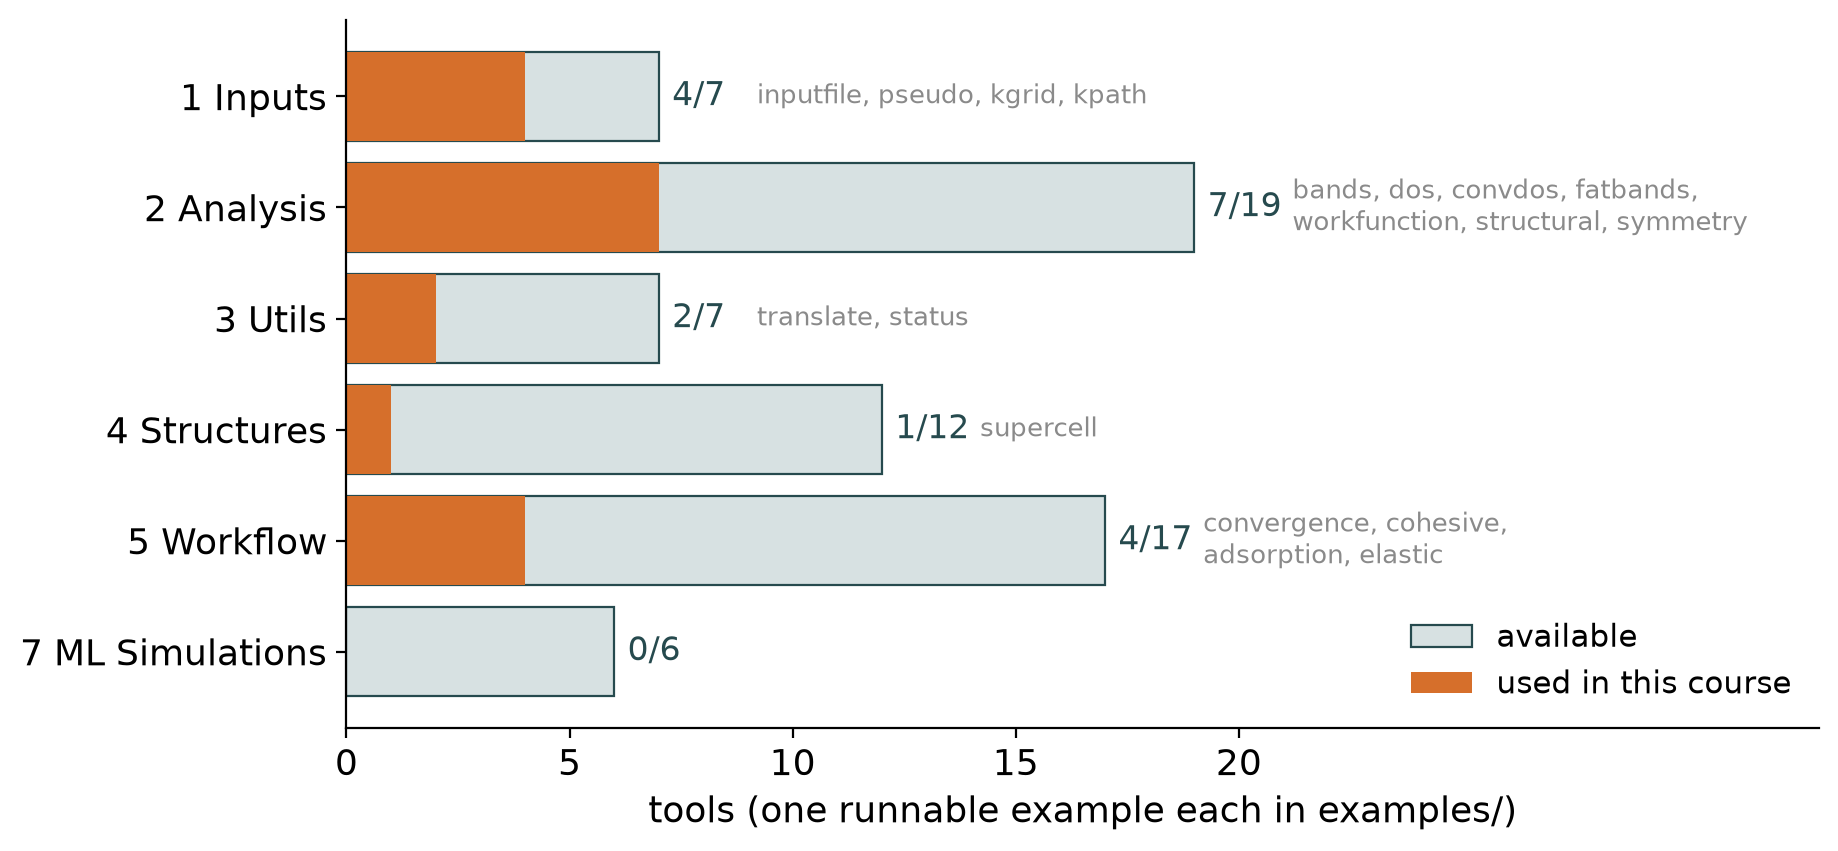
\includegraphics[width=0.88\textwidth]{figures/stb_coverage.png}
	\par\vspace{0.1cm}
	\begin{columns}[T]
		\begin{column}{0.48\textwidth}
			{\small \textbf{\color{stbteal}Natural next steps:} \texttt{5.1} strain,
			\texttt{5.15} equation of state, \texttt{5.4} phonons, \texttt{5.9} NEB,
			\texttt{2.6} Bader, \texttt{2.14} COOP.}
		\end{column}
		\begin{column}{0.48\textwidth}
			{\small \textbf{\color{stbteal}Fast preview:} \texttt{7.4 stb-mlelastic},
			\texttt{7.6 stb-mladsorb} with a MACE potential before spending DFT time.}
		\end{column}
	\end{columns}
\end{frame}

%-------------------------------------------------
% SLIDE 2.7.6 - Where to go next
%-------------------------------------------------
\begin{frame}[fragile]{Where to Find Everything}
	\begin{columns}[T]
		\begin{column}{0.52\textwidth}
			\metroset{block=fill}
			\begin{block}{STB-Suite}
				\small
				Docs: \texttt{stb-suite.github.io/stb}\\
				Code: \texttt{github.com/stb-suite/stb}\\[3pt]
				{\scriptsize
\begin{verbatim}
stb-suite        # menu: type a code, e.g. 5.2.1
stb-<tool> --help
examples/<code>-<tool>/README.md
\end{verbatim}
				}
				{\scriptsize Every tool has a guide and a runnable example script.}
			\end{block}
		\end{column}
		\begin{column}{0.44\textwidth}
			\metroset{block=fill}
			\begin{block}{Course material}
				{\footnotesize
\begin{verbatim}
aula1/
  relaxation/  convergence/
  cohesive_energy/
aula2/
  bandas_dos/
  fatbands_workfunction/
  adsorption/
  elastic/
\end{verbatim}
				}
			\end{block}
		\end{column}
	\end{columns}
	\vspace{0.1cm}
	\metroset{block=fill}
	\begin{alertblock}{Same layout in every example}
		\small
		\begin{itemize}
			\item \texttt{run/} or \texttt{input/}: start here
			\item \texttt{siesta\_stage*\_complete/}: SIESTA done, ready for the next STB stage
			\item \texttt{complete/}: final results, to compare with yours
		\end{itemize}
	\end{alertblock}
\end{frame}

%-------------------------------------------------
% SLIDE 2.7.7 - Questions
%-------------------------------------------------
\begin{frame}[standout]
	Questions?
	\par\vspace{0.6cm}
	{\normalsize\mdseries prepare $\rightarrow$ run $\rightarrow$ analyze $\rightarrow$ question the number}
\end{frame}


\begin{frame}{Acknowledgments}
	\begin{center}
		\large
		First, I would like to thank the \textbf{SEEDMOL COMMITE},
		for the invitation.

		\vspace{0.6cm}

		I gratefully acknowledge the funding agencies.
		I also thank the national HPC centers \textbf{Santos Dumont/LNCC} and \textbf{CENAPAD}.

		\vspace{0.5cm}

		\begin{columns}[c]
			\column{0.25\textwidth}
			
\includegraphics[width=\linewidth]{figures/cnpq.png}
			\column{0.25\textwidth}
			
\includegraphics[width=\linewidth]{figures/fapdf.png}
			\column{0.25\textwidth}
			
\includegraphics[width=\linewidth]{figures/capes.jpg}
		\end{columns}
	\end{center}
\end{frame}

\begin{frame}{University of Brasilia}
	Laboratório de Computação em Ciência de Materiais (LCCMat)
	\vspace{1cm}
	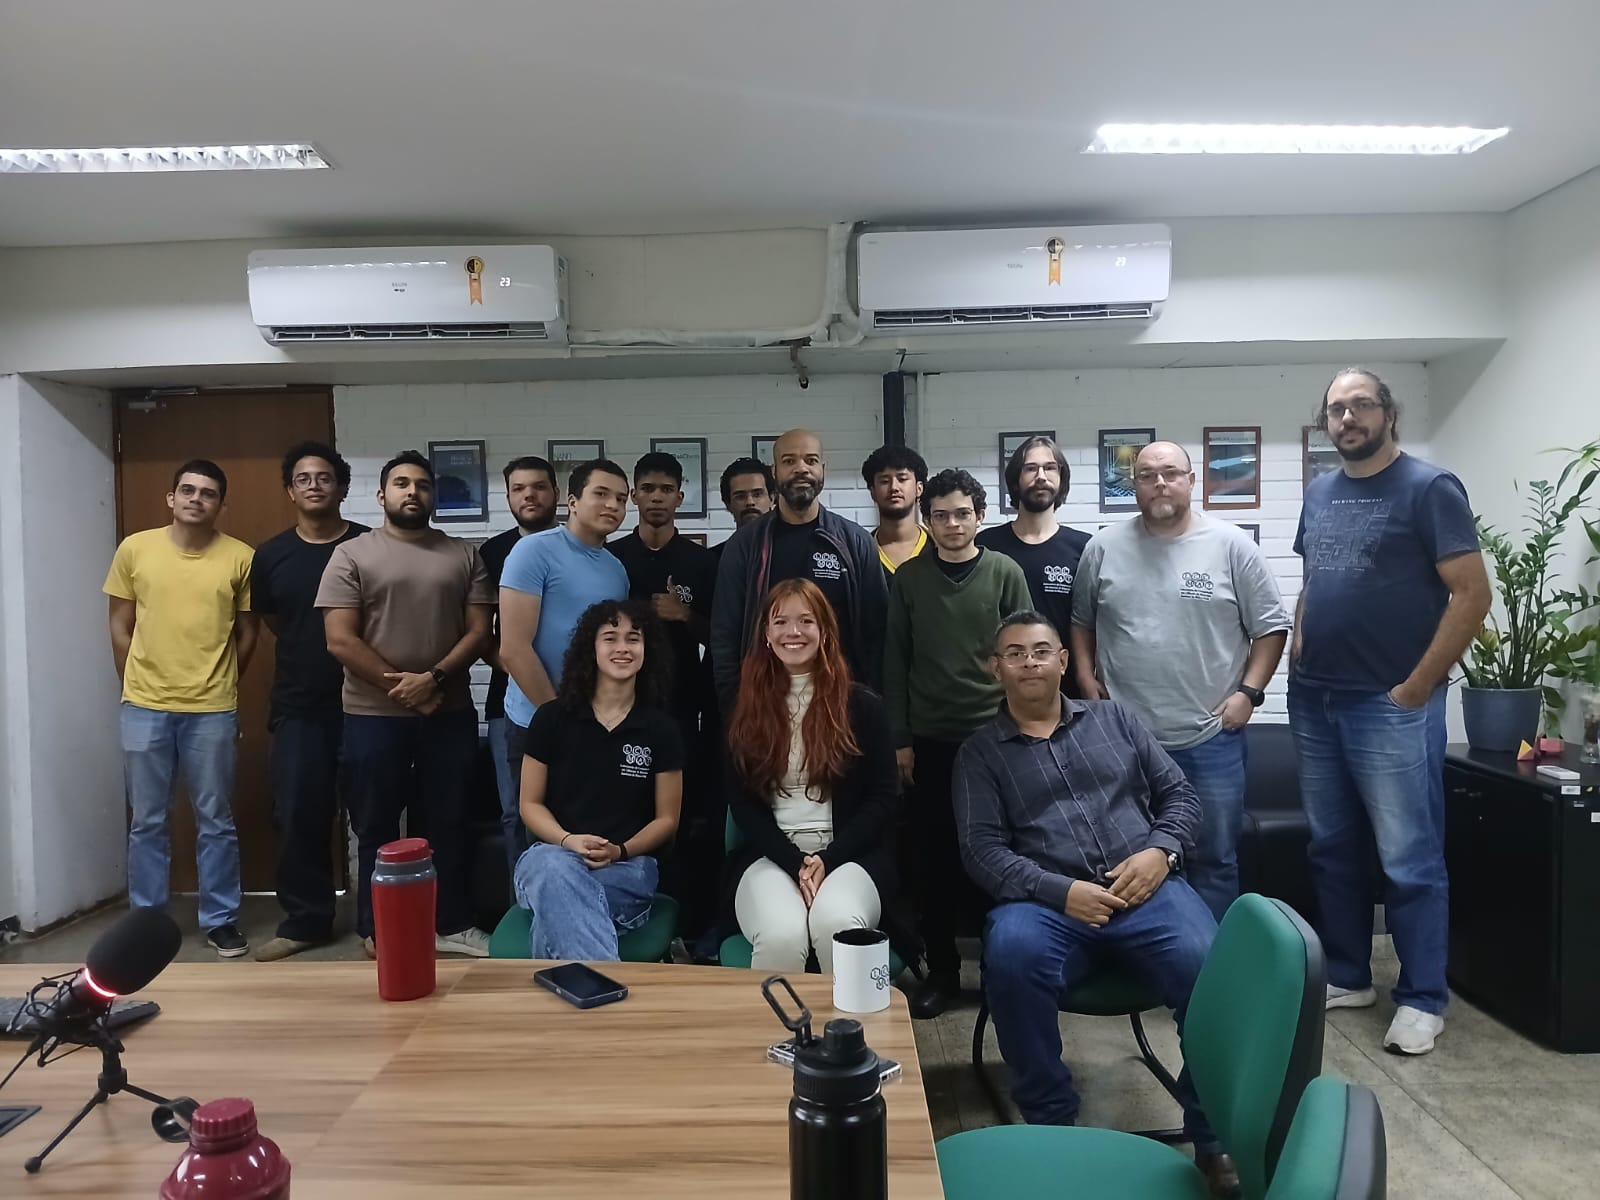
\includegraphics[width=\textwidth]{figures/lccmat.jpeg}
\end{frame}

% --- CONTACT & THANK YOU SLIDE ---
\begin{frame}
\frametitle{Thank You \& Let's Connect!}
\begin{columns}[c] % 'c' for vertically centered columns

    \column{0.4\textwidth}
        \centering
        % This QR code will generate a mailto link
        \qrcode[height=4cm]{https://bastoscmo.github.io/}
        \vspace{0.5cm}

        \large{my email: carlos.bastos@unb.br}

    \column{0.6\textwidth}
        \large
        We're always open to new collaborations...

        \vspace{0.7cm}

        ...especially if they involve discussing physics over a good cup of coffee!

	
\includegraphics[height=3cm]{figures/cofee.png}

        \vspace{1cm}

        \huge{\textbf{Thank you!}}

\end{columns}
\end{frame}

\end{document}
